\documentclass[a4paper, 11pt]{book}
\usepackage[T1]{fontenc}
\usepackage[utf8]{inputenc}
\usepackage[french]{babel}
\usepackage[]{palatino}
\usepackage[]{graphicx}
    \setkeys{Gin}{width=\linewidth}
    \graphicspath{./Captures}
\usepackage[]{float}
    \floatplacement{figure}{H}
    \floatplacement{table}{H}
\usepackage[table]{xcolor}
	\rowcolors{1}{white!95!black}{white}
\usepackage{multicol}
\usepackage[]{hyperref}
    \hypersetup{
        colorlinks=true,
        linkcolor=blue,
        urlcolor=blue!50!purple,
    }
    \urlstyle{same}
\usepackage[]{array}
%\usepackage[margin=35mm]{geometry}
\usepackage[all, defaultlines=3]{nowidow}
\usepackage[Sonny]{fncychap}
\title{Formation Apps.education}
\author{F.S.G.}
\date{Compilation du \today{}.}
\renewcommand{\baselinestretch}{1.25}
\setlength{\parskip}{0.5em}
\begin{document}
\begin{titlepage}
    \maketitle
\end{titlepage}

% chapitre d'introduction
\chapter*{Introduction}
\addcontentsline{toc}{chapter}{Introduction}

Suite --ou en parallèle-- de la formation dispensée au collège, ce livret dont la vocation est de servir aussi bien de trame formative mais aussi de guide de référence au long terme puisqu'au fur et à mesure des révisions ce livret sera enrichi de nombreux chapitres consacrés aux applications indidividuelles présentes ou s'intégrant au bouquet de service offert sur apps.

Il est aussi possible de contribuer à l'élaboration du livre puisqu'il est présent sur un dépôt \emph{github} dont l'adresse figure à la fin de cet ouvrage. 

Où trouver de l'information ? C'est relativement simple, elle est disponible sur les salons du réseau social \textbf{tchap} dédiés à \emph{apps} : \url{https://matrix.to/#/#apps.education.fr:agent.education.tchap.gouv.fr} ouvert à toutes celles et ceux pouvant accéder au réseau.

Par choix, j'ai décidé d'articuler ce document de la manière suivante~:
\begin{itemize}
	\item cette introduction,
	\item la genèse et un court historique du projet,
	\item la connexion au service, que le compte soit déjà créé ou non,
	\item un survol sommaire des différents services logiciels proposé au sein du bouquet numérique,
	\item l'examen plus approfondi et précis des possibilités offertes par le nuage
	\item l'examen plus précis de chaque application au fur déjà présente
	\item viendront ensuite s'ajouter les examens plus précis des nouvelles applications ajoutées ...
	\item une table des contenus --chapitres, sections, fiches pratiques ...-- 
	\item les remerciements et informations légales
\end{itemize}

\paragraph*{Participation.}
Le choix qui a été fait est de privilégier des langages d'écritures textuels les plus purs possibles, excluant \emph{de facto\/} les documents compressés bureautiques classiques (.doc, .docx, .odt). 
Cependant, dans un esprit de bienveillance et d'accueil des bonnes volontés, si vous savez enregistrer vos documents en ``document plat XML'' --disponibles avec \emph{Office} de Microsoft et \emph{libreoffice} de la Document Foundation-- ou bien, que dans un effort de formation vous vous initiez à l'utilisation de langages très simples tels que \emph{Markdown}\footnote{%
Descriptif du langage : \url{https://fr.wikipedia.org/wiki/Markdown} ; Un descriptif des quelques balises de formatage \url{https://www.ionos.fr/digitalguide/sites-internet/developpement-web/markdown/} et une petite leçon sur ce langage \url{https://programminghistorian.org/fr/lecons/debuter-avec-markdown}
}

Sinon, il est possible simplement de soumettre des modifications textuelles brutes en précisant le fichier à modifier, les lignes à rectifier et les modifications à apporter, ce qui est déjà une participation pertinente.

Vous pourrez retrouver une version en cours de développement de ce guide sur mon dépôt \emph{GitHub} à l'adresse \url{https://github.com/fgonz666/FormationApps}.

% Inclusion dans l'introduction : révisions du document
\section{Révisions du document}
\begin{table}
	\centering
	\renewcommand{\arraystretch}{1.25}
	\begin{tabular}{| m{0.15\linewidth} | m{0.1\linewidth} | m{0.15\linewidth} | m{0.55\linewidth} |}
		\hline
		Date & n$^0$ de version & Auteur principal & Modifications apportées \cr
		\hline
		2022-06-15 & 0.01 & F.S.G. & Création du document (Markdown) \cr
		\hline
		2022-06-17 & 0.02 & F.S.G. & Passage Markdown $\rightarrow$ \LaTeX{} \newline Plan modifié \cr
		\hline
		2022-06-18 & 0.03 & F.S.G. & Document monolithique $\rightarrow$ documents séparés pour une meilleure répartition des tâches et une lecture simplifiée. \cr
		\hline
		2022-06-20 & 0.04 & F.S.G. & Modification de la numérotation, ajout de nouvelles captures et de paragraphes sur l'utilisation du nuage. \cr
		\hline
		2022-06-24 & 0.05 & F.S.G. & Ajouts divers dans l'utilisation du nuage, tant en contenu et en structure.
		\newline Ajout d'une nouvelle capture d'écran sur CodiMD. \cr
		\hline
		2022-06-25 & 0.06 & F.S.G. & Modifications dans la partie libreoffice d'utiliser le nuage
		\newline Ajout d'une capture d'écran sur libreoffice writer. \cr
		\hline
	\end{tabular}
\end{table}


\paragraph{Objectif} : Initier les collègues à l'utilisation du portail apps mis en place par notre ministère pour tous les agents qu'ils soient en académie ou en administration centrale. 

\vspace{2cm}

Cette formation et son livret d'accompagnement s'organisent suivant le plan suivant~:
\begin{itemize}
    \item Création du compte
    \item Présentation des services
    \item Présentation plus détaillée du \emph{cloud\/}.
\end{itemize}


% chapitre historique
\chapter*{Un peu d'histoire}
\addcontentsline{toc}{chapter}{Un peu d'histoire}

\emph{Apps} est un projet initié en 2017 par les équipes du ministère (Bureau B1-1 de la direction du Numérique Éducatif) pour proposer aux agents un environnement numérique  moderne et répondant aux usages des utilisateurs, dans le cadre du projet SNP (Service Numériques Partagés). 
En effet la fragmentation des usages liée au nombre important des membres de l'éducation nationale --estimés dans le rapport à 1,2 millions d'agents dont environ 900~000 enseignants et 300~000 non-enseignants--, la diversité des métiers --une centaine répertoriés-- et par conséquent des usages rend difficile de proposer un outil unique avec un usage monolithique. 
Le choix d'un agréggateur de services permettant à chacun d'activer les services correspondant à ses usage a été alors préféré.

Ce projet a été ensuite récupéré par le bureau \og~Socle Numérique~\fg{} afin d'offrir aux agents des outils numériques de travail collaboratif mais toujours avec l'optique d'outils numérique, collaboratifs et accessibles sur le lieu de travail ou à l'extérieur, domicile compris. ``Un commun pour les agents''.

Le service centralisateur, appelé ``La Boite'',  est situé ici : \url{https://portail.apps.education.fr}



% chapitre de connexion et de création d'un compte
\chapter{Se connecter à ou créer son compte}
%\addcontentsline{toc}{chapter}{Se connecter à ou créer son compte}

\section{La première connexion}
La première chose à faire est de se connecter au site du portail qui est situé à \url{https://portail.apps.education.fr} comme le montre la capture d'écran suivante~:
\begin{figure}
    \centering
    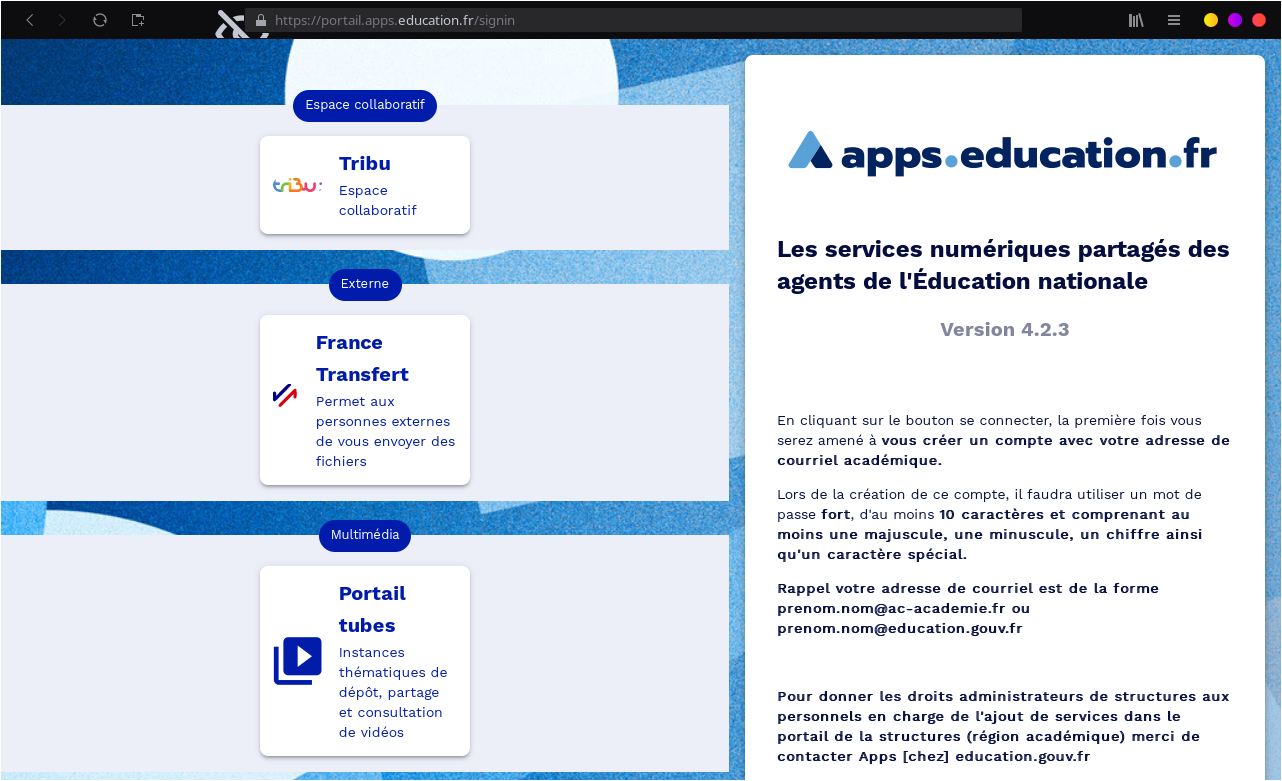
\includegraphics{Captures/portail.site.web.png}
\end{figure}

En bas à gauche se trouve le bouton \fbox{\hspace{1cm}SE~CONNECTER\hspace{1cm}} il donne alors accès à la fenêtre de connexion qui suit. 
\begin{figure}
	\centering
	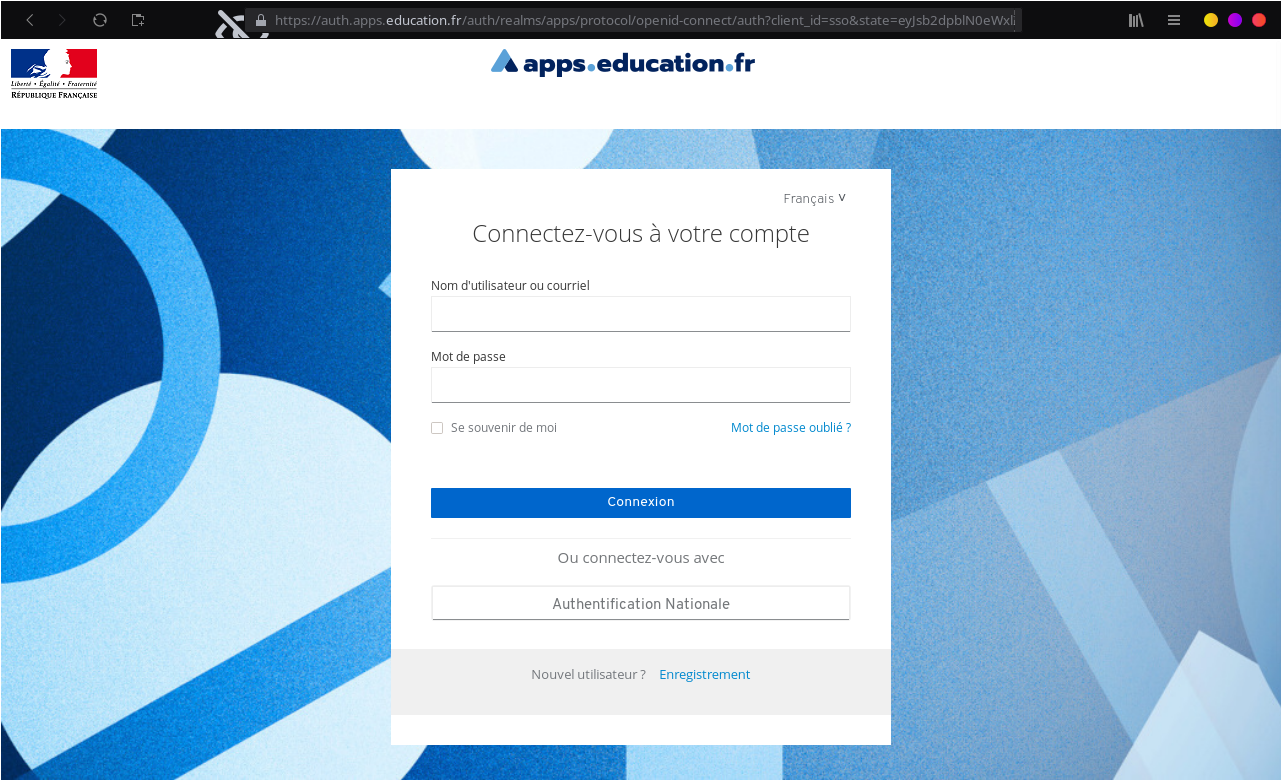
\includegraphics{./Captures/portail.site.web.connexion.png}
\end{figure}

Si on y regarde de plus près, on voit qu'on peut s'y connecter en saisissant son adresse professionnelle (académique ou ministérielle) mais également via un nom d'utilisateur. 
\begin{figure}
	\centering
	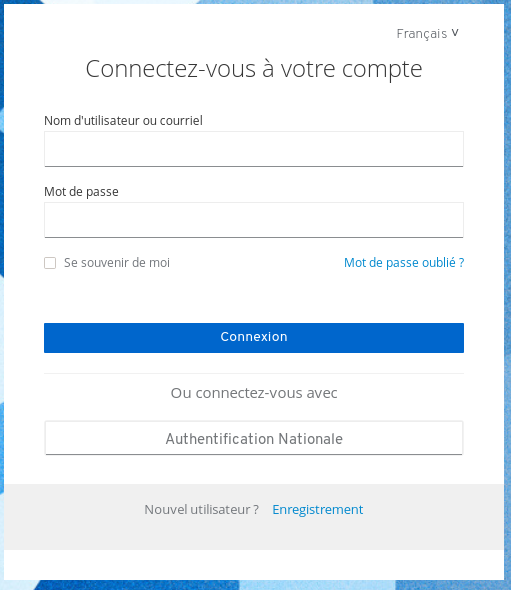
\includegraphics[width=0.500\linewidth]{./Captures/portail.site.web.connexion.zoom.png}
\end{figure}
Vers le bas de la fenêtre, une connexion avec ``Authentification Nationale'' est proposée, cette authentification sera abordée dans un \emph{attendum} ultérieur.

Évidemment la première fois impossible d'utiliser cette fenêtre de connxion puisque ``La Boîte'' ne nous connaît pas, aussi, la présence en bas à droite du lien \href{https://auth.apps.education.fr/auth/realms/apps/login-actions/registration?client_id=sso&tab_id=bVmOhc3T6kQ}{Enregistrement} va permettre l'inscription au service et à compter de ce moment-là cette fenêtre de connexion suffira.

La fenêtre d'enregistrement, comme cette capture, montre la présence en quatrième ligne d'un champ dédié à l'identifiant, c'est là qu'il faudra l'inventer en suivant les règles demandées et précisées en dessous du chmap.
\begin{figure}
	\centering
	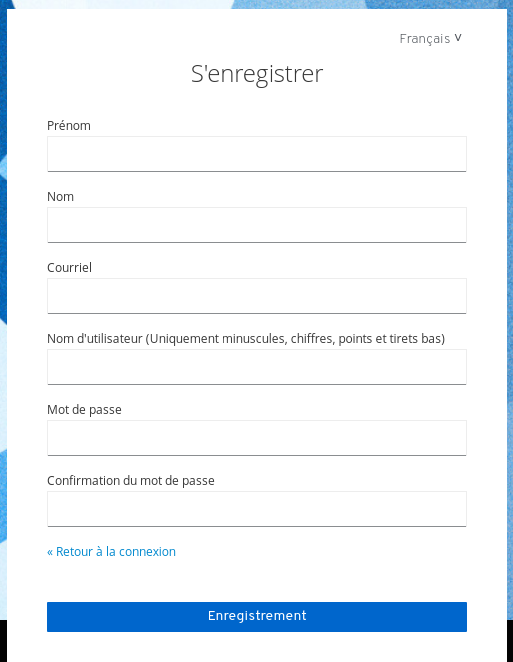
\includegraphics[width=0.500\linewidth]{./Captures/portail.site.web.enregistrement.png}
	\caption{}
\end{figure}

\paragraph{Avantage de l'identifiant.} Au cours d'une carrière nous sommes tous amenés à changer d'établissements, et une partie d'entre nous pour ne pas dire une majorité, nous changeons d'académie. 
Dès lors, le changement d'adresse mail s'opère pour chaque agent, et, comme l'intention de la boite est de rester un outil pérenne qui suit l'agent dans le temps, il faut pouvoir s'y connecter même en changeant de fonction ou d'académie, aussi la présence de cet identifiant vous permettra de vous connecter au compte et ensuite d'y modifier l'adressse mail de rattachement.

Une fois cette étape prête, un lien vers la fenêtre de confirmation sera envoyé à l'adresse de courriel précisée dans le formulaire précédent, soyez relativement rapides, ce lien arrive vite à expiration, je conseille d'ailleurs d'avoir ouvert sa messagerie avant la phase d'enregistrement pour s'assurer de la réception du lien par courriel et de l'activation au plus vite du profil.

\section{Derniers réglages du profil simplifié.}

\begin{figure}
	\centering
	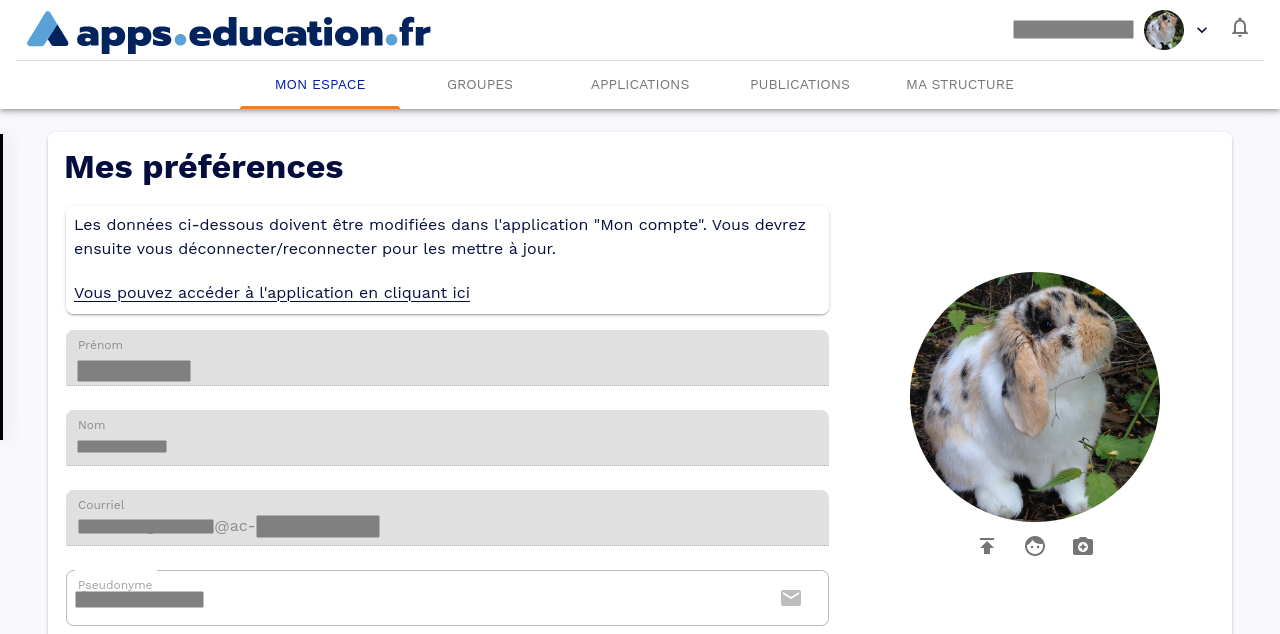
\includegraphics{./Captures/portail.profil.haut.png}
	\caption{}
\end{figure}

\begin{figure}
	\centering
	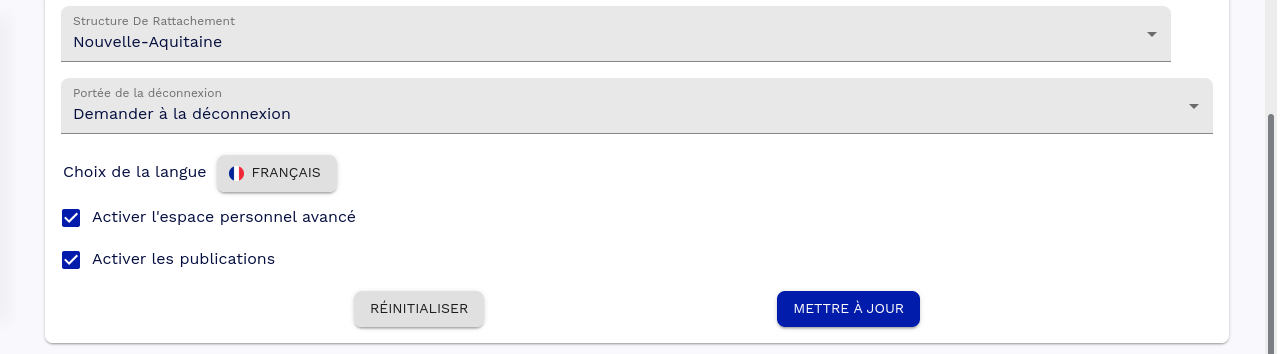
\includegraphics{./Captures/portail.profil.milieu.png}
	\caption{}
\end{figure}

\begin{figure}
	\centering
	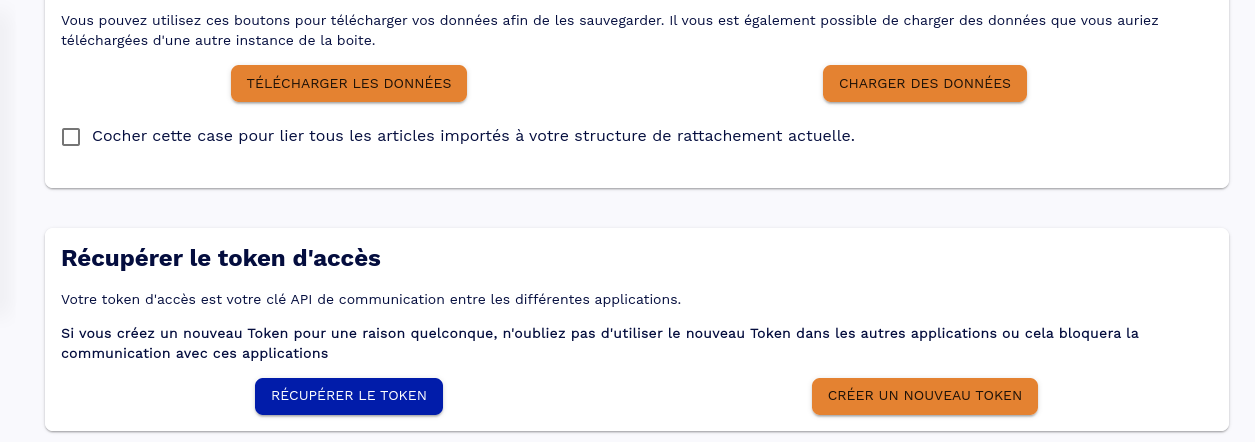
\includegraphics{./Captures/portail.profil.bas.png}
	\caption{}
\end{figure}

\section{Réglages fins du profil et augmentation de la sécurité.}

% Chapitre de découverte des services offerts
\chapter{Découvrir les différents services}
%\addcontentsline{toc}{chapter}{Découvrir les différents services}

Le portail est le centre névralgique de l'environnement de la Boîte. 
Au début il est pour ainsi dire vide sauf la présence dans l'espace, en haut, d'une barre avec plusieurs onglets~:
\begin{figure}
	\centering
	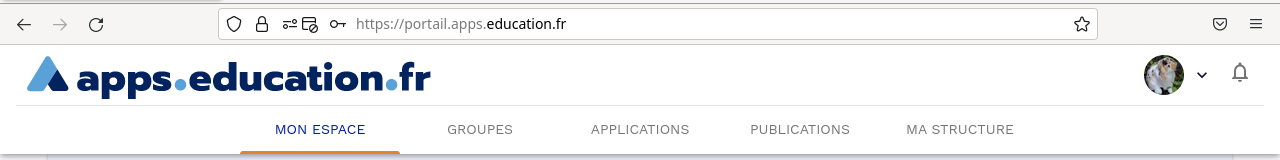
\includegraphics[width=\linewidth]{./Captures/portail.barre.haute.png}
%	\caption{}
\end{figure}
Une fois la première connexion établie, il sera demandé de vérifier et compléter le profil. 
De nombreux champs, ceux utilisés lors de l'enregistrement ne sont pas modifiables, et généralement il reste quelques options à régler en bas~: la structure de rattachement et les options de publication

Deux onglets seront intéressants dans les premiers temps, celui des groupes et celui des applications puisque leur rôle est d'ajouter de nouvelles vignettes au sein de l'accueil (onglet de gauche).

\begin{figure}
	\centering
	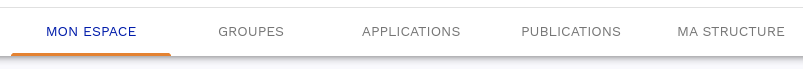
\includegraphics[width=\linewidth]{./Captures/portail.barre.seule.png}
%	\caption{}
\end{figure}

Une fois que vous aurez ajouté les applications ou les groupes, votre portail pourra évoluer et par exemple ressembler à celui-ci~:
\begin{figure}
	\centering
	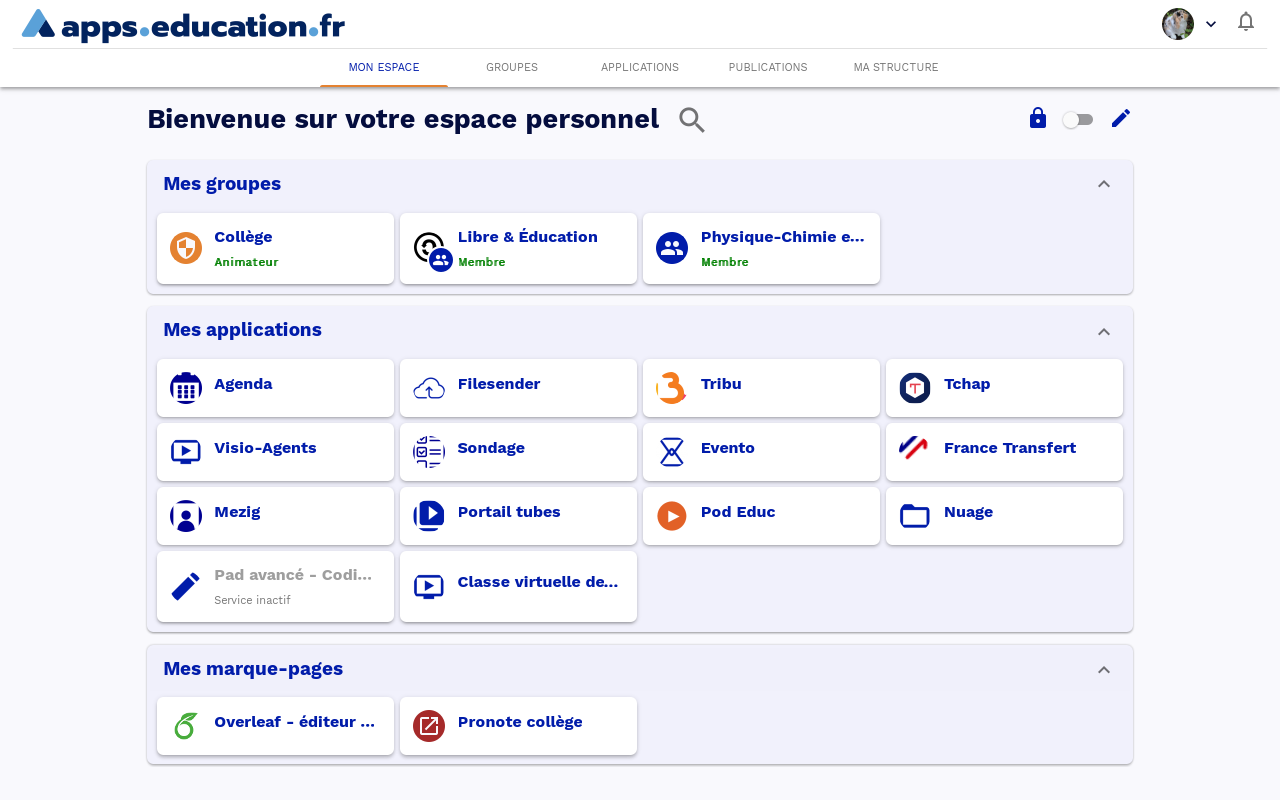
\includegraphics[width=0.7071\linewidth]{./Captures/portail.accueil.png}
%	\caption{}
\end{figure}

\paragraph*{Comment ajouter de nouvelles briques ?}
La méthode est assez simple, il suffit de jeter un \oe{}il soit aux onglets, soit au menu de l'utilisateur à droite.

% portail-ajout-groupe.tex
\section{Ajouter un groupe à son profil}

\subsection{Affichage de tous les groupes disponibles}
Une fois l'onglet \og~\bsc{groupes}~\fg{} sélectionné comme le montre la capture d'écran la liste des groupes disponibles, 193 ici au message \textbf{Explorer les groupes (193)}. 
À sa droite une loupe vous permet de saisir un mot clé du nom du groupe si vous le connaissez et le filtre agira en affichant uniquement les éléments concernés.
\begin{figure}
	\centering
	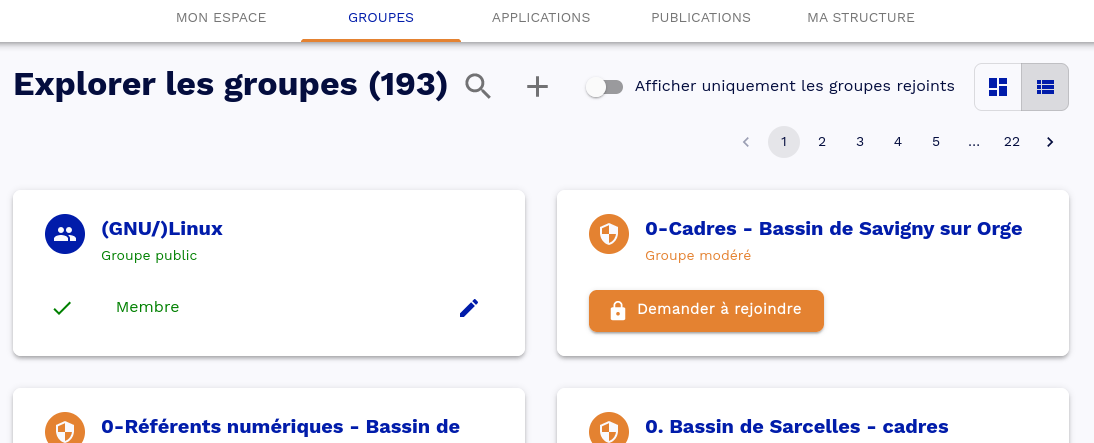
\includegraphics{./Captures/portail.groupes.selection.png}
	\caption{Affichage des différents groupes disponibles}
\end{figure}

À la droite de la loupe, un grand signe plus vous permet de créer un groupe, où, par défaut en tant que créateur, vous serez aussi l'administrateur.

\begin{quote}
	\emph{Là où l’on trouve un grand pouvoir, on trouve une grande responsabilité.}\newline
	\begin{flushright} Winston Churchill (1906) \end{flushright}
\end{quote}


\subsection{S'inscrire à un groupe}
Parmi les groupes se trouvent des groupes publics ouverts à tous, donc les accentuations colorées sont bleu où l'inscription est automatique dès que vous cliquez sur le bouton \fbox{$\boxed{\rightarrow}$ \hspace{0.1cm} Rejoindre le groupe}
\begin{figure}
	\centering
	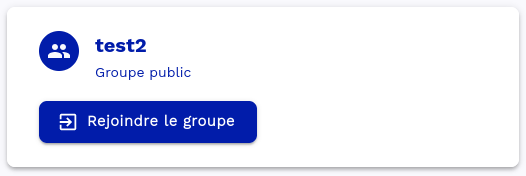
\includegraphics[width=0.500\linewidth]{Captures/portail.groupe.exemple.public.png}
	\caption{Exemple de groupe public}
\end{figure}
C'est le cas de ce groupe Test2 ou bien auparavant du groupe \textbf{(GNU)/Linux}, mais se trouvent aussi des groupes modérés à inscription suite à une validation, ces groupes apparaissent avec des icônes oranges circulaires représentant l'équivalent d'un bouclier, et aussi par une coloration orange. 
De même le bouton n'affiche pas \emph{Rejoindre le groupe} comme auparavant mais un cadenas et \textbf{Demander à rejoindre} puisqu'un modérateur ou un administrateur devra accepter l'inscription pour pouvoir accéder au groupe.

Si un icône a été défini pour le groupe, alors la coloration bleuté restera et l'icône du groupe s'affichera avec un icône générique (bleu ou orange) à ses côtés

\begin{figure}
	\centering
	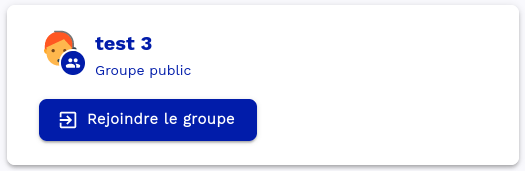
\includegraphics[width=0.500\linewidth]{./Captures/portail.groupe.exemple.public.avec.icone.png}
	\caption{Exemple de groupe public avec icône spécifique.}
\end{figure}

Il en va de même avec les groupes modérés évidemment.

une fois les groupes intéressants ajoutés au profil, ce dernier les affichera directement dans la zone ``\textbf{Mes groupes}'' dédiée aux groupes comme le montre la capture suivante.

\begin{figure}
	\centering
	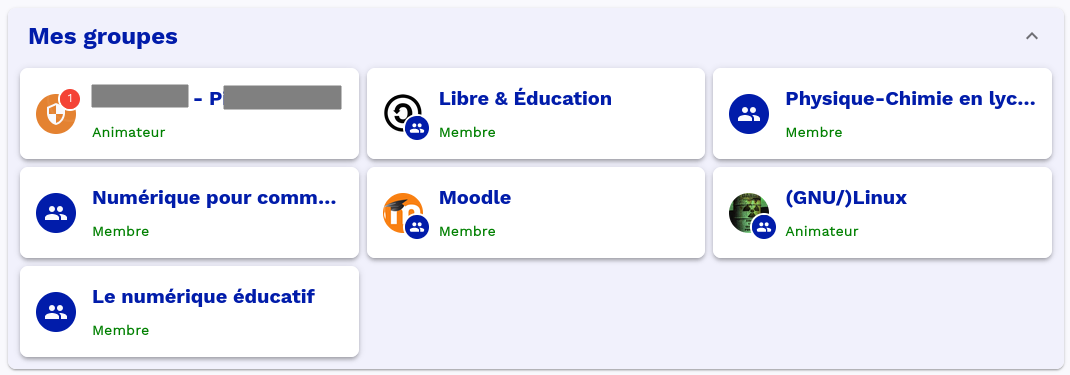
\includegraphics{./Captures/portail.accueil.mes.groupes.png}
	\caption{Les groupes ajoutés à mon profil.}
\end{figure}

Vous aurez noté sur le groupe du haut, à gauche, la présence d'un 1 dans un cercle rouge. 
Dans ce groupe modéré puisque de couleur orange où je suis animateur --comprendre administrateur-- il y a une notification. 
En l'occurrence il s'agit ...

\paragraph{Notez la présence d'un \^{} en haut à droite.}
Celui-ci permet de replier la zone consacrée à l'affichage de mes groupes.

\subsection{Gérer mes groupes}
La gestion des groupes s'effectue à partir du menu du profil. 
Bien évidemment, il s'agit de gérer les groupes dont on est administrateur ou modérateur, pas simple utilisateur
\begin{figure}
	\centering
	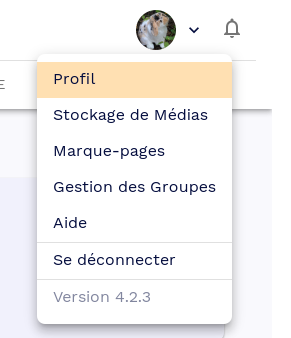
\includegraphics[width=0.3333\linewidth]{./Captures/menu.profil.png}
%	\caption{}
\end{figure}

\subsection{Détails d'un groupe}
En cliquant sur un des groupes, au hasard un de ceux administrés, voici les détails qui s'affichent. 
Ce tableau de bord complet montre tous les réglages et les options auxquelles il est possible d'accéder.
\begin{figure}
	\centering
	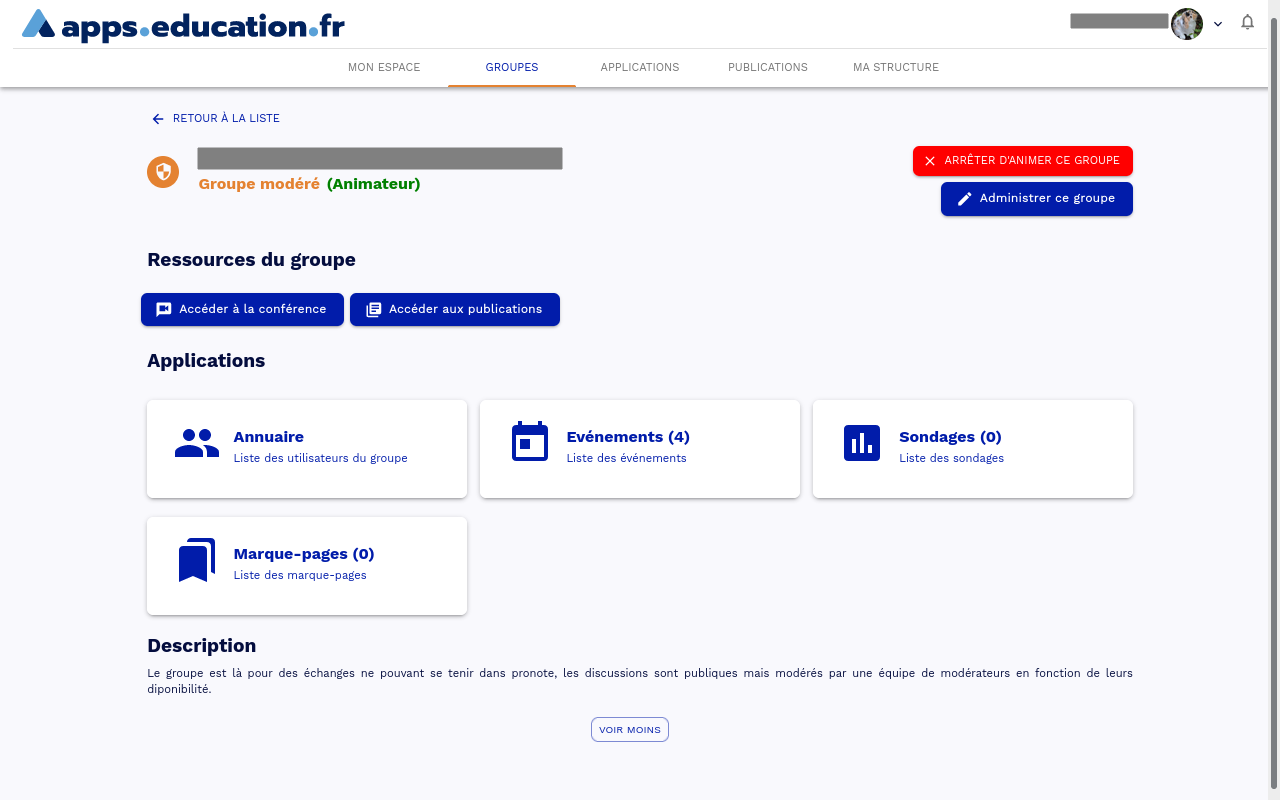
\includegraphics{./Captures/portail.groupe.affichage.details.png}
	\caption{L'intégralité des détails d'un groupe.}
\end{figure}


%%portail-ajout-application.tex
\section{Ajouter une application au profil}
Cette fois-ci c'est l'onglet \bsc{application} qui devra être sélectionnée.
\begin{figure}
	\centering
	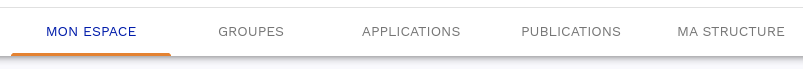
\includegraphics[width=\linewidth]{./Captures/portail.barre.seule.png}
%	\caption{}
\end{figure}
Dès lors, la liste des applications disponible apparaît avec des icônes permettant de filtrer par centre d'intérêt.
\begin{figure}
	\centering
	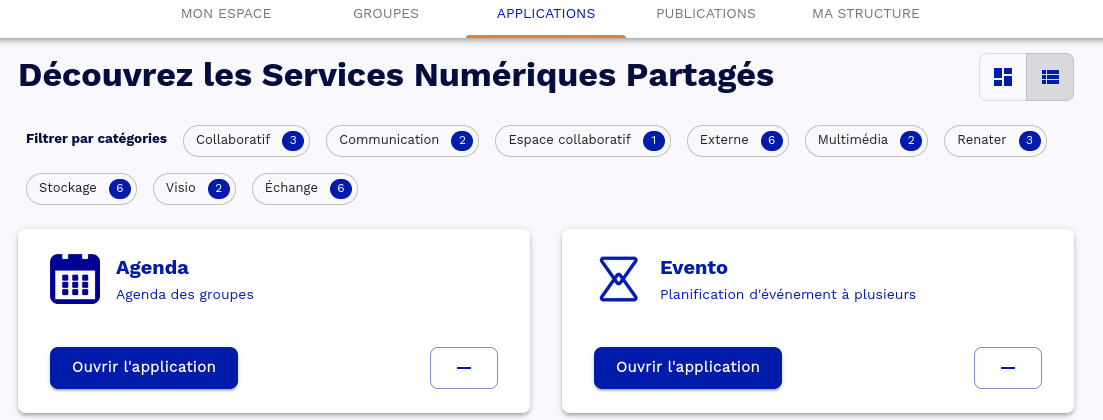
\includegraphics{./Captures/portail.applications.selection.png}
	\caption{sélectionner des applications}
\end{figure}
La capture précédente montre que les deux applications, \textbf{Agenda} et \textbf{Evento} sont déjà ajoutées à mon profil car sinon l'icône en bas à droite serait un ``+'' pour l'ajouter, alors que là c'est un ``--'' qui est visible me permettant de retirer l'application du profil.
\begin{figure}
 	\centering
 	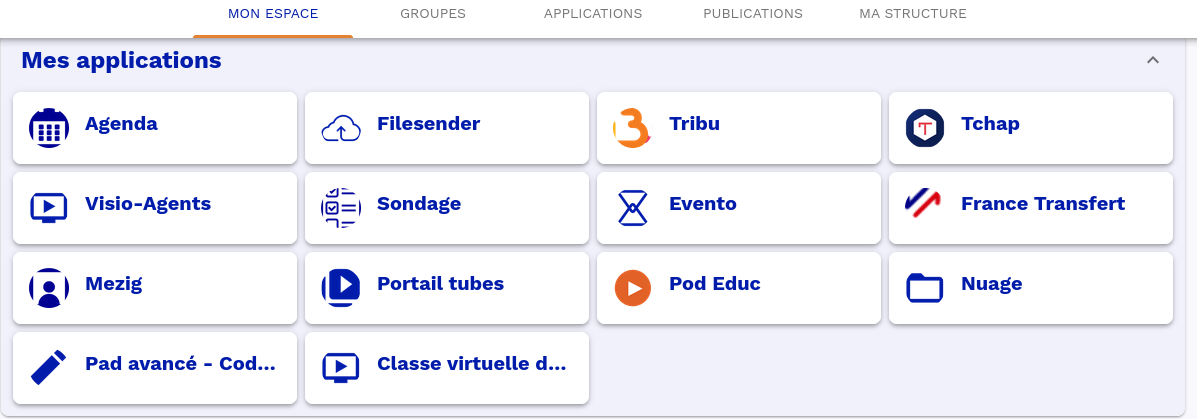
\includegraphics{./Captures/portail.mes.applications.png}
 	\caption{Les applications visibles et accessibles dans mon profil.}
 \end{figure}
Il est évidemment possible de retirer toute application du profil lorsque l'envie vous prendra.

% portail-ajout-bookmarks.tex
\section{Ajouter des liens extérieurs}
Parfois certaines applications en ligne ne sont pas pensées pour être intégrée au sein du projet Apps. 
Dans mon cas, le lien vers notre outil de gestion des notes, bulletins, cahiers de textes et absences, ou encore un environnement de développement de documents en \LaTeX{} n'est pas non plus disponible, mais, grâce à l'outil d'ajout de bookmarks, il est possible de les intégrer au sein du portail.

Comme pour la gestion des groupes, tout va commencer sur le menu du profil en haut à droite.
\begin{figure}
	\centering
	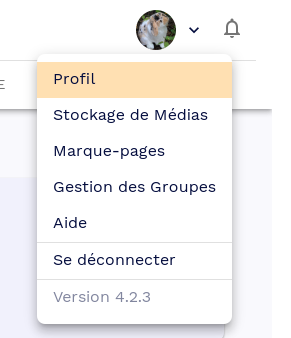
\includegraphics[width=0.3333\linewidth]{./Captures/menu.profil.png}
%	\caption{}
\end{figure}
et cette fois-ci c'est le choix ``Marque-pages'' qui va être choisi. 

\subsection{Descriptif de la fenêtre}
Une fois la ligne cliquée, une zone ressemblant à cet espace, mais vide bien sûr au début, va s'afficher. 
En voici un descriptif rapide.
\begin{figure}
	\centering
	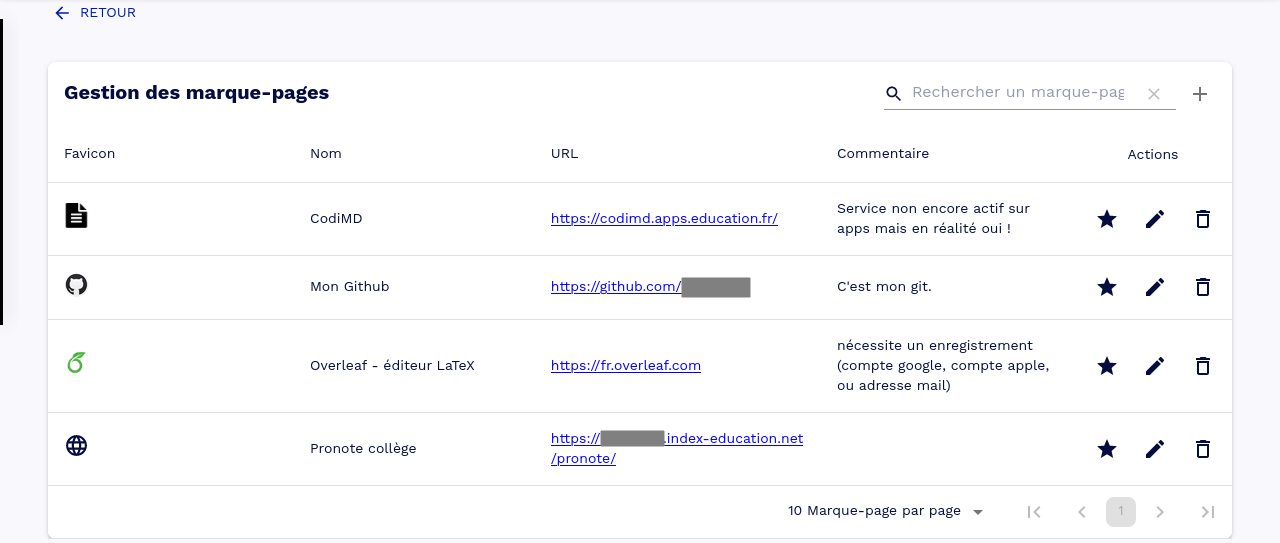
\includegraphics{./Captures/portail.marque.pages.gestion.png}
	\caption{Les marque-pages actuellement saisis dans mon profil}
\end{figure}
\begin{itemize}
	\item Situé en haut à gauche un lien de Retour permet de revenir à l'accueil,
	\item En haut vers la droite, un champ de recherche avec une loupe à sa droite permet de retrouver un lien si vous avez de nombreux liens déjà enregistrés,
	\item tout à droite, un + permet la création d'un nouveau marque page,
	\item la zone centrale affiche, ligne à ligne chaque marque page, les détails sont expliqués là $\rightarrow$ \ref{subsec-detail-bookmark},
	\item en bas à droite une ligne de navigation permet d'aller de page en page ou d'en sélectionner une lorsque beaucoup de liens auront été ajoutés et qu'ils ne tiendront plus sur une ligne unique.
\end{itemize}

\subsection{Détails d'un marque page} \label{subsec-detail-bookmark}
Voici l'examen détaillé d'une ligne de marque-pages, l'exemple du lien vers le site \emph{overleaf}.
\begin{figure}
	\centering
	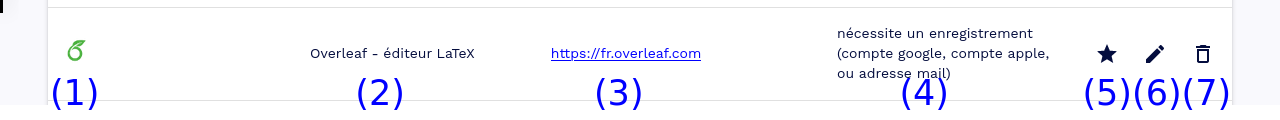
\includegraphics{./Captures/portail.marque.pages.exemple.png}
	\caption{Un exemple de marque-page, vers le site Overleaf}
\end{figure}
La ligne comporte sept zones différentes, voici leur explication de gauche à droite.
\begin{enumerate}
	\item icône du site web en question, sinon un icône générique,
	\item nom donné par moi-même au marque page,
	\item adresse internet du site,
	\item descriptif saisi par moi-même lors de la création du marque page,
	\item marque cet élément comme devant être parmi les favoris donc présent dans la page d'accueil, si l'étoile est creuse, le marque page reste ici, si elle est pleine, alors non seulement il sera présent dans la liste mais aussi apparaîtra en bas de l'onglet d'accueil,
	\item le stylo permet de modifier ultérieurement les détails du marque-page saisis lors de sa création,
	\item comme on peut aisément le deviner, l'icône poubelle permet d'effacer le marque-page, la capture suivante montre d'ailleurs le résultat.
\end{enumerate}
\begin{figure}
	\centering
	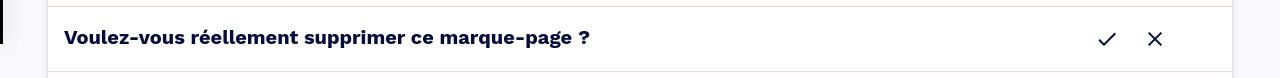
\includegraphics{./Captures/portail.marque.pages.suppression.png}
	\caption{Suppression d'un marque page en attente de ma validation}
\end{figure}
L'appui sur $\surd$ validera l'action de suppression, sur $\times$ vous aurez simplement le retour à la liste des marque pages sans suppression.

De retour à l'écran d'accueil, vous aurez, en bas du profil, tous les marque-pages marqués comme favoris apparaissent.
\begin{figure}
	\centering
	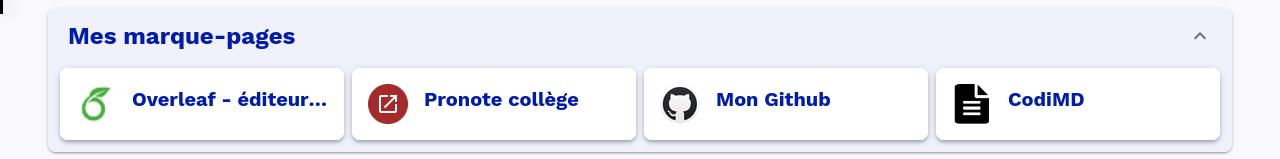
\includegraphics{./Captures/portail.accueil.mes.favoris.png}
	\caption{Mes marque-pages favoris affichés dans le profil.}
\end{figure}

\subsection{Création d'un marque-pages}
En cliquant sur le ``+'' à droite de la zone de recherche, elle-même en haut à droite de la fenêtre, cette mini fenêtre va s'afficher centralement.
\begin{figure}
	\centering
	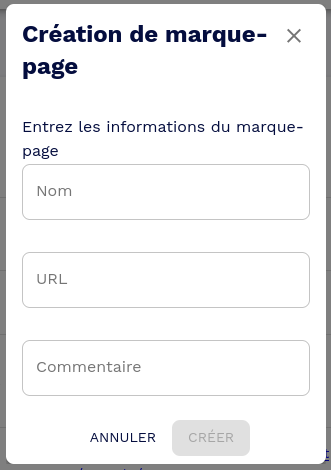
\includegraphics[width=0.333\linewidth]{./Captures/portail.marque.pages.creation.png}
	\caption{Création d'un marque page, pour l'instant vide.}
\end{figure}
Les seules indications importantes consistent à bien remplir tous les champs d'une part et surtout de bien ajouter \texttt{https://} ou \texttt{http://} en début d'adresse, le plus simple étant de copier-coller l'adresse affichée dans la barre éponyme du navigateur internet.

% portail-ajout-media.tex
\section{Ajouter des médias au profil}
En passant par la ligne de \textbf{stockage des média}, vous accéderez à une page spécifique montrant toutes les images que vous souhaitez stocker dans votre profil, hors du nuage étudié dans le chapitre idoine. 
Notez deux limitations :
\begin{itemize}
	\item l'espace maximum alloué est 100~Mo,
	\item chaque item ne peut pas dépasser la taille limite de 3~Mo
\end{itemize}
\begin{figure}
	\centering
	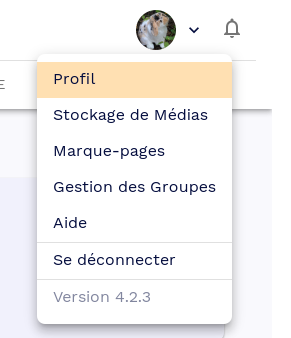
\includegraphics[width=0.3333\linewidth]{./Captures/menu.profil.png}
%	\caption{}
\end{figure}

\subsection{Ajouter un média}
Il existe deux méthodes pour ajouter un media à cet espace, le plus facile est d'ouvrir une fenêtre de l'explorateur de fichiers devant le navigateur, d'y sélectionner un ou plusieurs éléments, puis de les faire glisser sur la fenêtre du navigateur, les fichiers seront alors ajoutés à la liste des éléments présents.

L'autre méthode consiste à appuyer sur l'icône + à droite de la fenêtre, vers le haut.
\begin{figure}
	\centering
	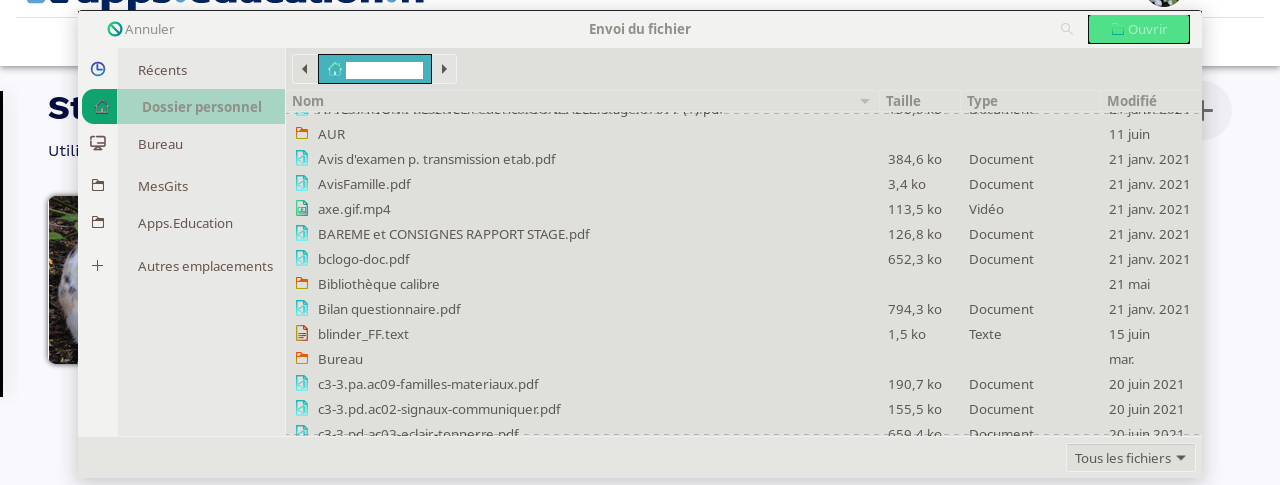
\includegraphics{./Captures/portail.stockage.medias.explorateur.png}
	\caption{L'appui sur ``+'' ouvre le navigateur local, ici en négatif car thème sombre originalement.}
\end{figure}
Une fenêtre de l'explorateur s'ouvrira, invitant l'utilisateur à choisir des éléments pour les y monter, comme le montre la capture plus haut
\begin{figure}
	\centering
	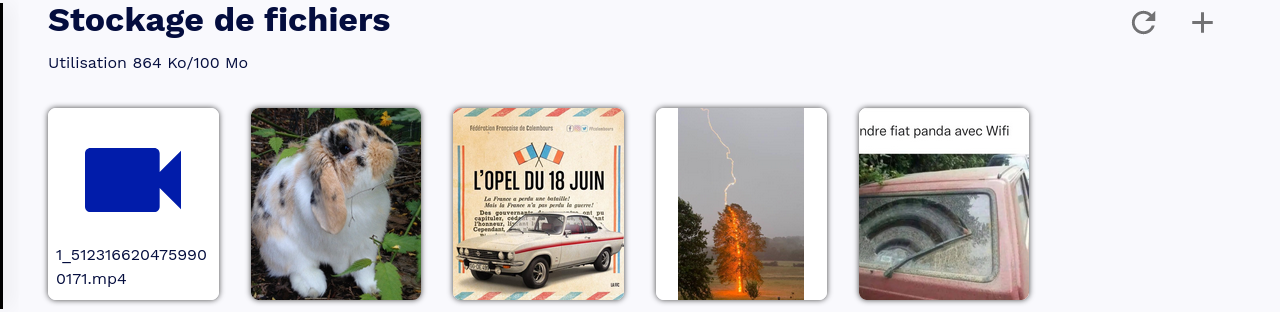
\includegraphics{./Captures/portail.stockage.medias.exemples.png}
	\caption{Affichage de quelques exemples déjà stockés sur mon profil.}
\end{figure}

\subsection{Gérer un média}
En sélectionnant un média, une mini-fenêtre de visualisation partielle (pour les images) ou de lecture (pour les vidéos) apparaît, elle se présente comme l'exemple qui suit.
\begin{figure}
	\centering
	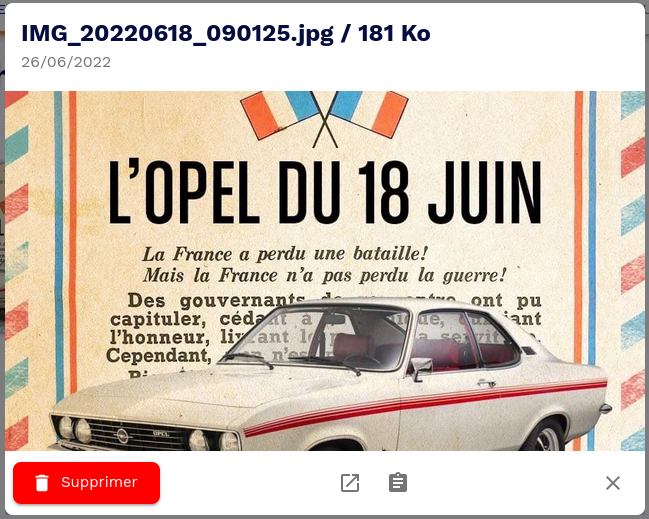
\includegraphics[width=0.500\linewidth]{./Captures/portail.stockage.medias.exemple.seul.png}
	\caption{Affichage d'un exemple de média stocké.}
\end{figure}
Vous aurez noté en haut le nom et la taille du document, quant à la partie basse elle présente une barre de gestion.
\begin{figure}
	\centering
	
\includegraphics[width=0.500\linewidth]{./Captures/portail.stockage.medias.barre.gestion.png}
	\caption{Les options de gestion d'une image stockée.}
\end{figure}
La barre de gestion des média affiche 4 options, de gauche à droite~:
\begin{itemize}
	\item un gros bouton rouge pour supprimer le média,
	\item un icône permettant d'afficher --sur mon navigateur cela déclenche le téléchargement-- du média dan sa totalité,
	\item un icône permettant de copier l'adresse de ce média,
	\item une croix pour fermer cette fenêtre.
\end{itemize}

\paragraph{Suppression d'un media.}
La suppression d'un média n'est pas directe et nécessite une double confirmation, en appuyant sur le gros bouton rouge, un compte à rebours de trois seconde s'enclenche pour valider cette suppression. 
À la fin du délais, si un second clic n'est pas venu attester le choix, la suppression n'est pas effective.
\begin{figure}
	\centering
	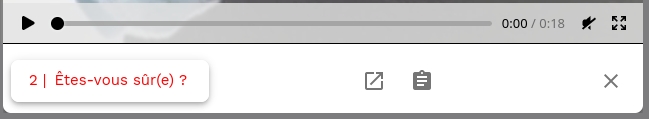
\includegraphics[width=0.500\linewidth]{./Captures/portail.stockage.medias.suppression.png}
	\caption{Suppression d'un média, êtes-vous sûr(e) ?}
\end{figure}


% portail-publications.tex
\section{Mes publications.}
Dans l'onglet \bsc{publications} sont regroupées toutes les publications que vous avez rédigées, publications forcément associées à un groupe.
\begin{figure}
	\centering
	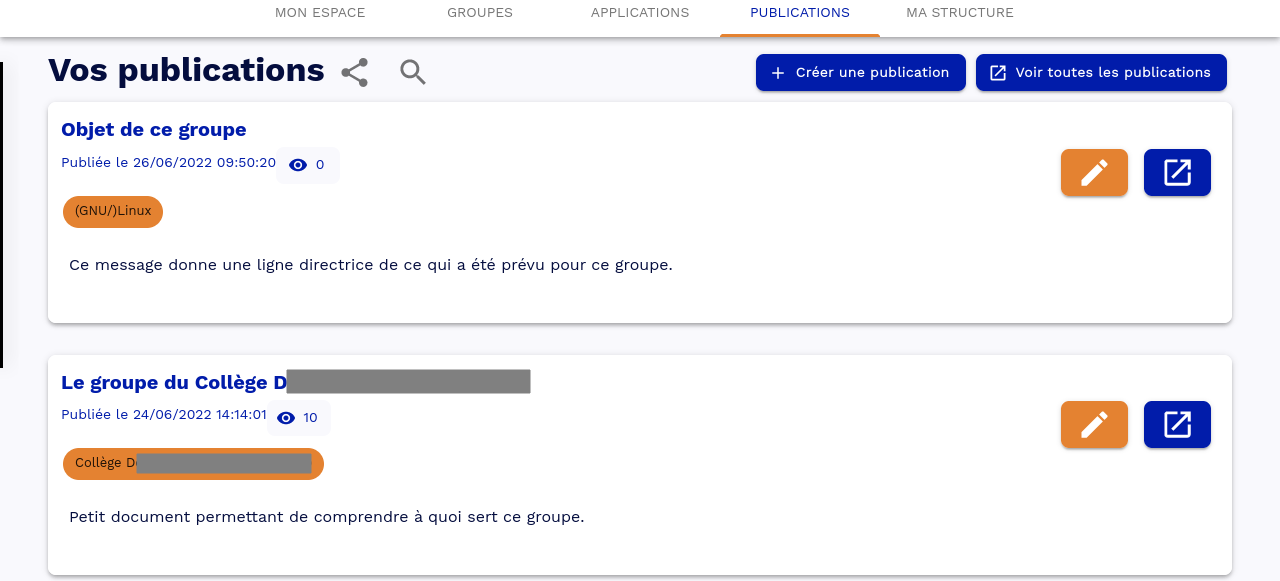
\includegraphics{./Captures/portail.publications.exemples.png}
	\caption{Exemples de publications personnelles.}
\end{figure}
Les seules options importantes sont regroupées vers la droite, il s'agit des gros boutons bleus pour
\begin{itemize}
	\item[+] Créer une publication
	\item[$\square$] Voir toutes les publications
\end{itemize}

Au sein d'une ligne de publication, les deux icônes importantes sont l'icône orange pour modifier une publication déjà rédigée, et pour afficher cette publication

\subsection{Créer une publication}
Lors de l'appui sur le bouton de création, une nouvelle fenêtre s'ouvre et les différents champs apparaissent. 
\begin{figure}
	\centering
	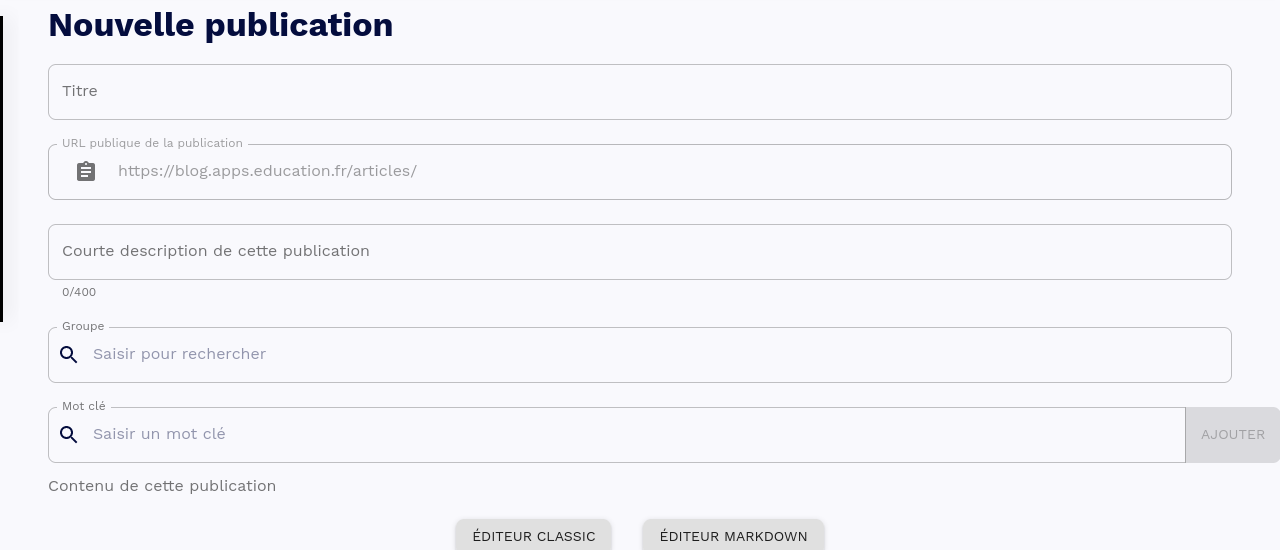
\includegraphics{./Captures/portail.publications.creer.publication.1.png}
	\caption{La première partie lors de la création d'une publication.}
\end{figure}
Parmi eux certains sont forcément obligatoires, en l'occurrence le titre bien sûr mais également le groupe dans lequel cette publication apparaîtra.

La partie inférieure de la fenêtre affiche deux options pour la publication et des boutons correspondants, à savoir l'éditeur classique ou l'éditeur markdown.

\paragraph{L'éditeur classique} affiche une barre d'options de formatage et d'inclusion d'objets classiques comme des listes numérotées ou pucées, des  permet aussi l'insertion d'en-têtes dans la publication (titre, sous-titre,  ...)
\begin{figure}
	\centering
	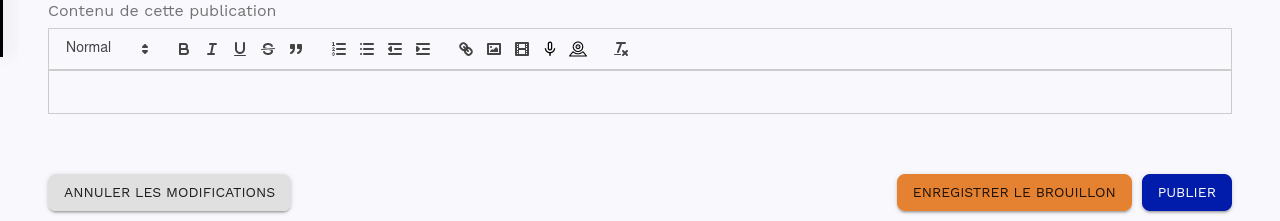
\includegraphics{./Captures/portail.publications.creer.publication.2.classique.png}
	\caption{La seconde partie de la création d'une publication : l'éditeur classique}
\end{figure}
De gauche à droite les icônes permettent :
\begin{itemize}
	\item de structurer le texte sélectionné avec un niveau hiérarchique dans le document,
	\item de mettre la sélection en (on peut cocher plusieurs choix)
		\begin{itemize}
		\item gras
		\item italique
		\item souligné
		\item barré
		\end{itemize}
	\item d'ajouter une citation
	\item d'ajouter une liste numérotée
	\item d'ajouter une liste pucée
	\item de diminuer le retrait du texte sélectionné
	\item d'augmenter le retrait du texte sélectionné
	\item d'ajouter un lien vers une ressource sur internet,
	\item d'insérer une image
	\item d'insérer une vidéo
	\item d'insérer un fichier audio
	\item d'enregistrer et insérer une vidéo (si la webcam existe sur l'ordinateur)
	\item de supprimer les mises en forme de la sélection
\end{itemize}

\paragraph{L'éditeur Markdown}
Markdown est un langage de balisage léger permettant de l'insertion d'objets et du formatage. 
Le chapitre \ref{chap-codimd} se réfère à ce langage tellement pratique qu'il est devenu mon outil de prise de notes pendant les réunions.
\begin{figure}
	\centering
	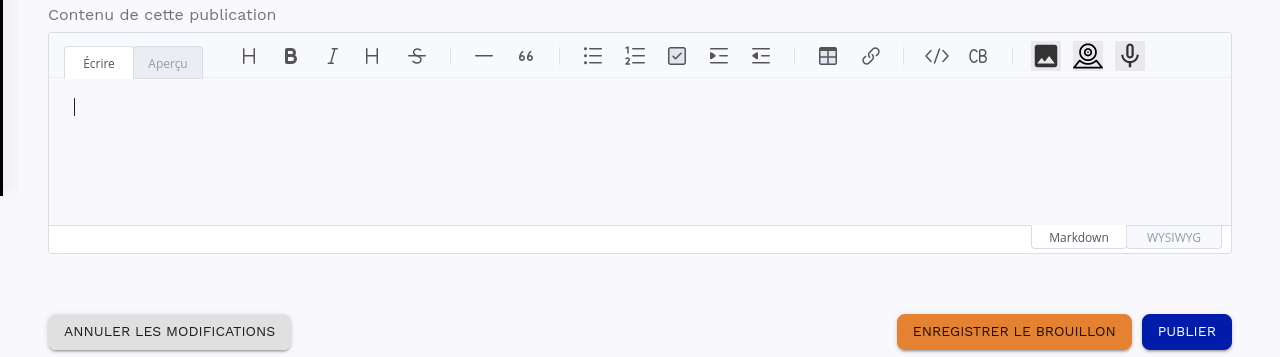
\includegraphics{./Captures/portail.publications.creer.publication.2.markdown.png}
	\caption{}
\end{figure}

\paragraph{Les deux modes acceptés en Markdown.} 
Ce sont le mode Markdown et le mode WYSIWYG\footnote{%
WYSIWYG : \emph{What You See Is What You Get} est un acronyme désignant une famille d'outils numériques, généralement des traitements de textes, où vous avez le formatage et le rendu en même temps que vous le saisissez. 
Cette famille diffère d'autres langages ou logiciels de traitement de texte comme Markdown, Restructured Text ou encore \TeX{} et \LaTeX{} (entre autres) où le formatage est signifié par des balises mais le rendu n'est visible qu'après compilation du document.
}.

L'éditeur Markdown offre la barre suivante avec de gauche à droite~:
\begin{figure}
	\centering
	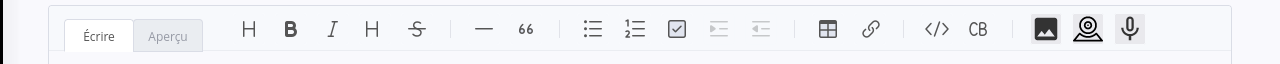
\includegraphics{./Captures/portail.publications.creer.publication.barre.markdown.png}
	\caption{L'éditeur Markdown}
\end{figure}
\begin{itemize}
	\item gestion des en-têtes (titre, sous-titre, ...), 
	\item gras,
	\item italique,
	\item choix de la couleur du texte,
	\item texte barré,
	\item ligne horizontale,
	\item citation,
	\item liste pucée,
	\item liste numérotée,
	\item case de tâche à cocher,
	\item augmentation du retrait du texte,
	\item diminution du retrait du texte,
	\item insertion d'un tableau,
	\item insertion d'un lien vers l'extérieur,
	\item insertion d'un code en ligne,
	\item insertion d'un code en bloc,
	\item ajout d'un media (comprendre image),
	\item enregistrement et ajout d'une vidéo,
	\item enregistrement et ajout d'une séquence audio
\end{itemize}

L'éditeur WYSIWYG offre la barre suivante, certaines options de l'éditeur markdown sont soit absentes, soit inactives (grisées clairement)
\begin{figure}
	\centering
	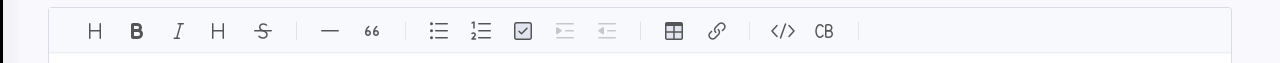
\includegraphics{./Captures/portail.publications.creer.publication.barre.wysiwyg.png}
	\caption{L'éditeur Markdown-Wysiwyg}
\end{figure}

\paragraph{Enregistrement}
Une fois la note saisie entièrement le bas de la fenêtre offre trois choix, celui de l'annulation, celui de l'enregistrement en tant que brouillon ou bien celui de la publication, comme le montre la capture suivante.
\begin{figure}
	\centering
	
\includegraphics{./Captures/portail.publications.creer.publication.3.png}
	\caption{\emph{this is your last chance}}
\end{figure}

\subsection{Voir toutes les publications}
L'autre bouton important de l'onglet publications ouvre une nouvelle fenêtre, ou un nouvel onglet suivant la configuration de votre navigateur, pour afficher les derniers articles du blog.
\begin{figure}
	\centering
	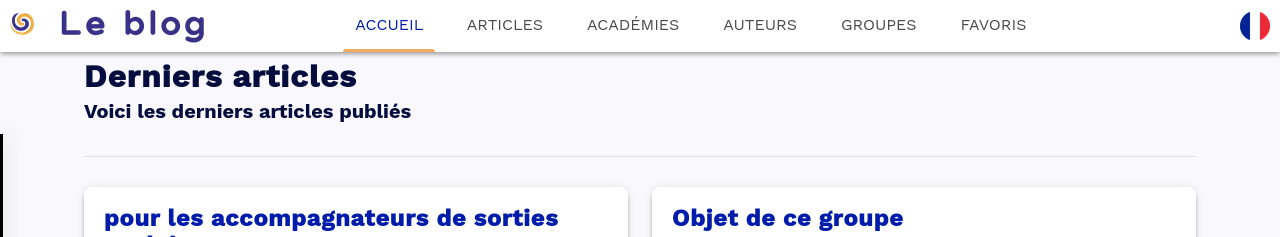
\includegraphics{./Captures/portail.publications.afficher.toutes.le.blog.png}
	\caption{Les derniers articles du blog}
\end{figure}

Notez que la barre du haut de la fenêtre est également changée, puisque cette fois-ci c'est celle qui suit qui s'affiche.
\begin{figure}
	\centering
	
\includegraphics{./Captures/portail.publications.afficher.toutes.le.blog.barre.png}
	\caption{La barre du blog}
\end{figure}
Elle permet d'afficher de gauche à droite, l'accueil avec les dernières publications, l'intégralité des publications avec un outil de filtrage par tags, les régions académiques avec les publications rattachées par région ou structure (comme CANOPÉ par exemple), la liste des auteurs et le nombre d'article qu'ils ont publié, la liste des groupes et le nombre de publications associées au groupe, et pour finir les publications lues et marquées comme favorites par vos soins.

% portail-structure.tex
\section{Ma structure}
Chaque structure régionale peut proposer des outils qui lui sont propres et intégrés au portail, cela se retrouvera dans l'onglet \bsc{ma structure}, ici la région nouvelle-aquitaine propose un outil de visioconférence, en cliquant sur le plus en bas à droite de la vignette (le plus devenant alors un moins) l'outil est ajouté au profil.
\begin{figure}
	\centering
	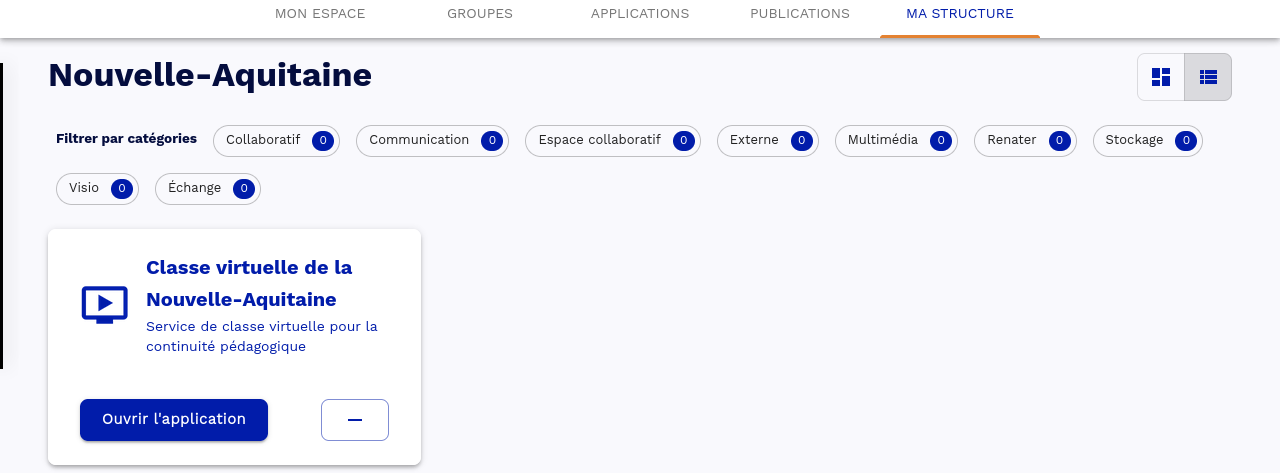
\includegraphics{./Captures/portail.accueil.ma.structure.png}
	\caption{Les applications et autres offres de la part de ma structure de rattachement.}
\end{figure}


Enfin, lorsque vous désirez quitter votre profil, surtout si vous êtes sur un ordinateur public, en passant par la dernière ligne du menu contextuel du profil, vous accéderez à la ligne de déconnexion. 
Celle-ci est primordiale pour une bonne hygiène informatique et quelques règles élémentaires de sécurité numérique.
\begin{figure}
	\centering
	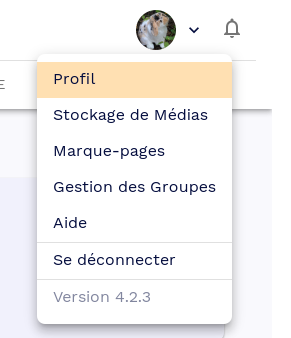
\includegraphics[width=0.3333\linewidth]{./Captures/menu.profil.png}
%	\caption{}
\end{figure}

% chapitre dédié au nuage
\chapter{Utiliser le nuage}
%\addcontentsline{toc}{chapter}{Utiliser le nuage}

Le ``Nuage'' est le nom qui a été donné à l'espace de stockage en ligne, actuellement d'une taille maximale de 100~Go\footnote{%
100~Go = 100 milliards de caractères simples.
} 
offrant en outre la présence d'une suite bureautique en ligne --libreoffice en ligne ou lool-- et d'éditeurs avancés de texte enrichi.

Le nuage est accessible de deux façons différentes pour l'instant --j'espère que la troisième fonctionnera aussi bientôt--~: \emph{via} l'interface web (firefox, chrome, edge, autres ...) ou \emph{via} le client \emph{nextcloud}.

Même si les avis divergent entre \emph{bloggers\/} au sein du vaste monde d'internet, il y a un adage que beaucoup partagent~: \og~\emph{There is no cloud : it's just someone else's computer.\/}\footnote{Il n'y a pas de Nuage : c'est seulement l'ordinateur de quelqu'un d'autre.}~\fg{}. 
En effet malgré que peut apporter un \emph{data center\/} ou un \emph{cluster} de telles structures en terme de répartition, si la société qui gère tout ce stockage distant décide de fermer le service, vous n'y aurez plus accès.

\section{L'interface Web}
%\addcontentsline{toc}{section}{L'interface web}

L'interface web est celle qui sera sans doute la plus utilisée car dès que l'on est en établissement scolaire, peu importe les blocages ou les applications, la certitude de trouver un navigateur dans chaque ordinateur est quasi absolue.
\begin{figure}
	\centering
	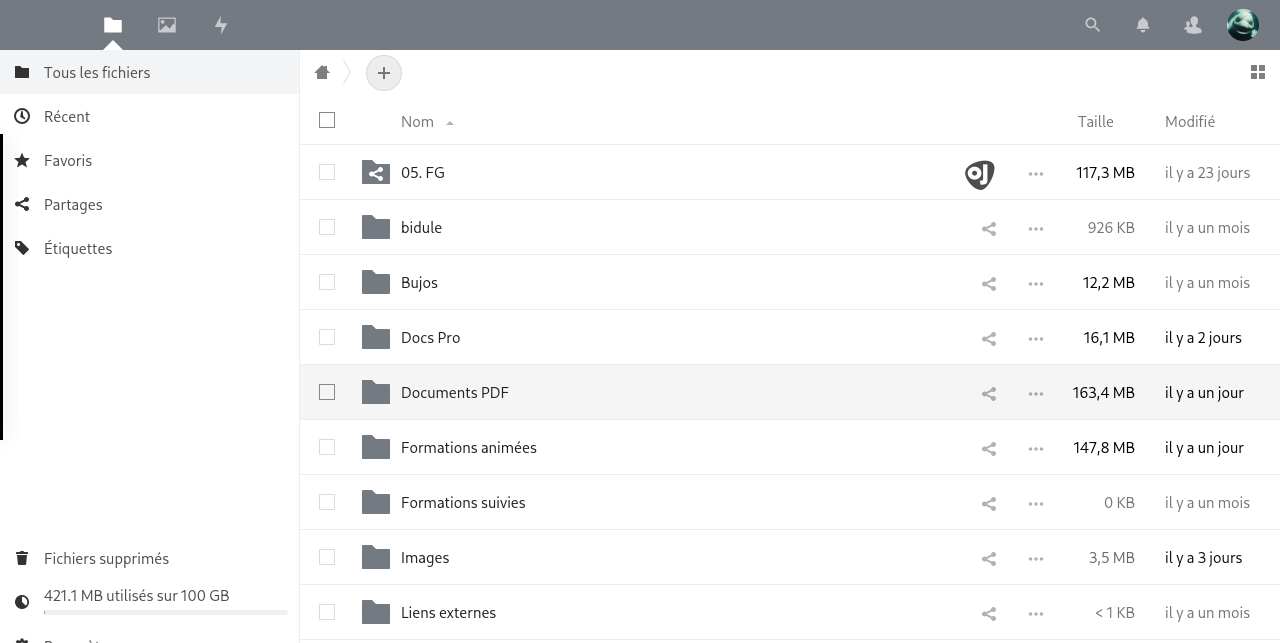
\includegraphics[width=\linewidth]{./Captures/nuage.accueil.png}
	\caption{Le nuage en mode détaillé}
\end{figure}
L'interface est visible en mode mosaïque également.
\begin{figure}
	\centering
	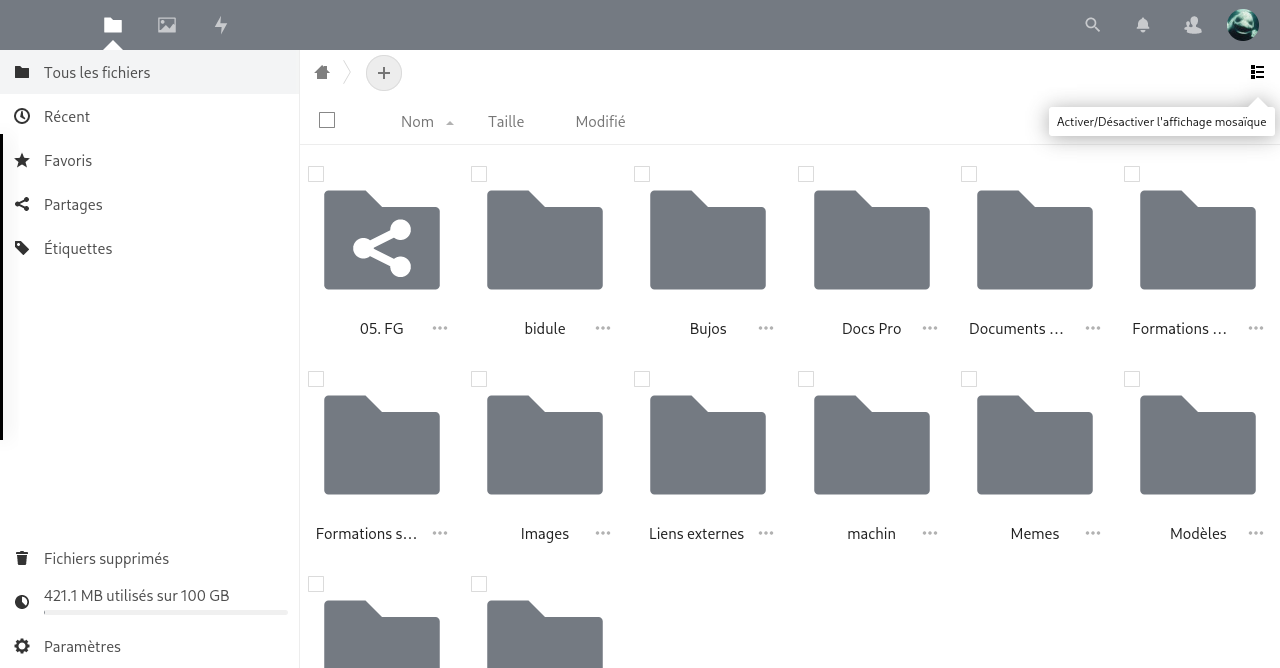
\includegraphics[width=\linewidth]{./Captures/nuage.accueil.mozaique.png}
	\caption{Le nuage en mode mosaïque.}
\end{figure}
L'intérêt de cette interface est de pouvoir y déposer ou récupérer un ou plusieurs fichiers, ou bien un ou plusieurs dossiers. 
L'autre intérêt est que le site étant en ``education.fr'' il ne sera donc pas filtré par les systèmes de pare-feu académiques et évitera l'emploi de clés USB qui se promènent entre le domicile et l'établissement où les niveau de sécurité sont très différents.



\section{Le client NextCloud}
%\addcontentsline{toc}{section}{Le client nextcloud}
Le nuage de \emph{apps} est basé sur le travail d'un groupe important de développeurs et de développeuses qui ont fondé le site et le serveur ``Nextcloud''. 
Ce service en ligne permet outre ce qui est offert par le nuage bien d'autres fonctionnalités. 

\begin{multicols}{2}

\begin{figure}
	\centering
	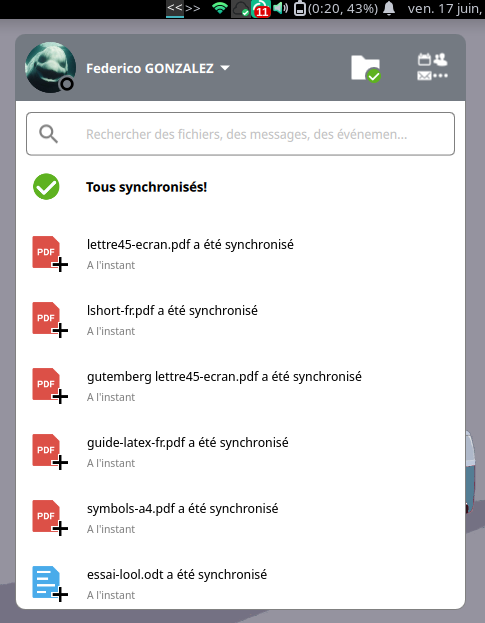
\includegraphics{./Captures/nextcloud-client.fenetre.principale.png}
	\caption{Le client pour PC (MacOS, Windows, ici : Linux}
\end{figure}

\columnbreak

\begin{figure}
	\centering
	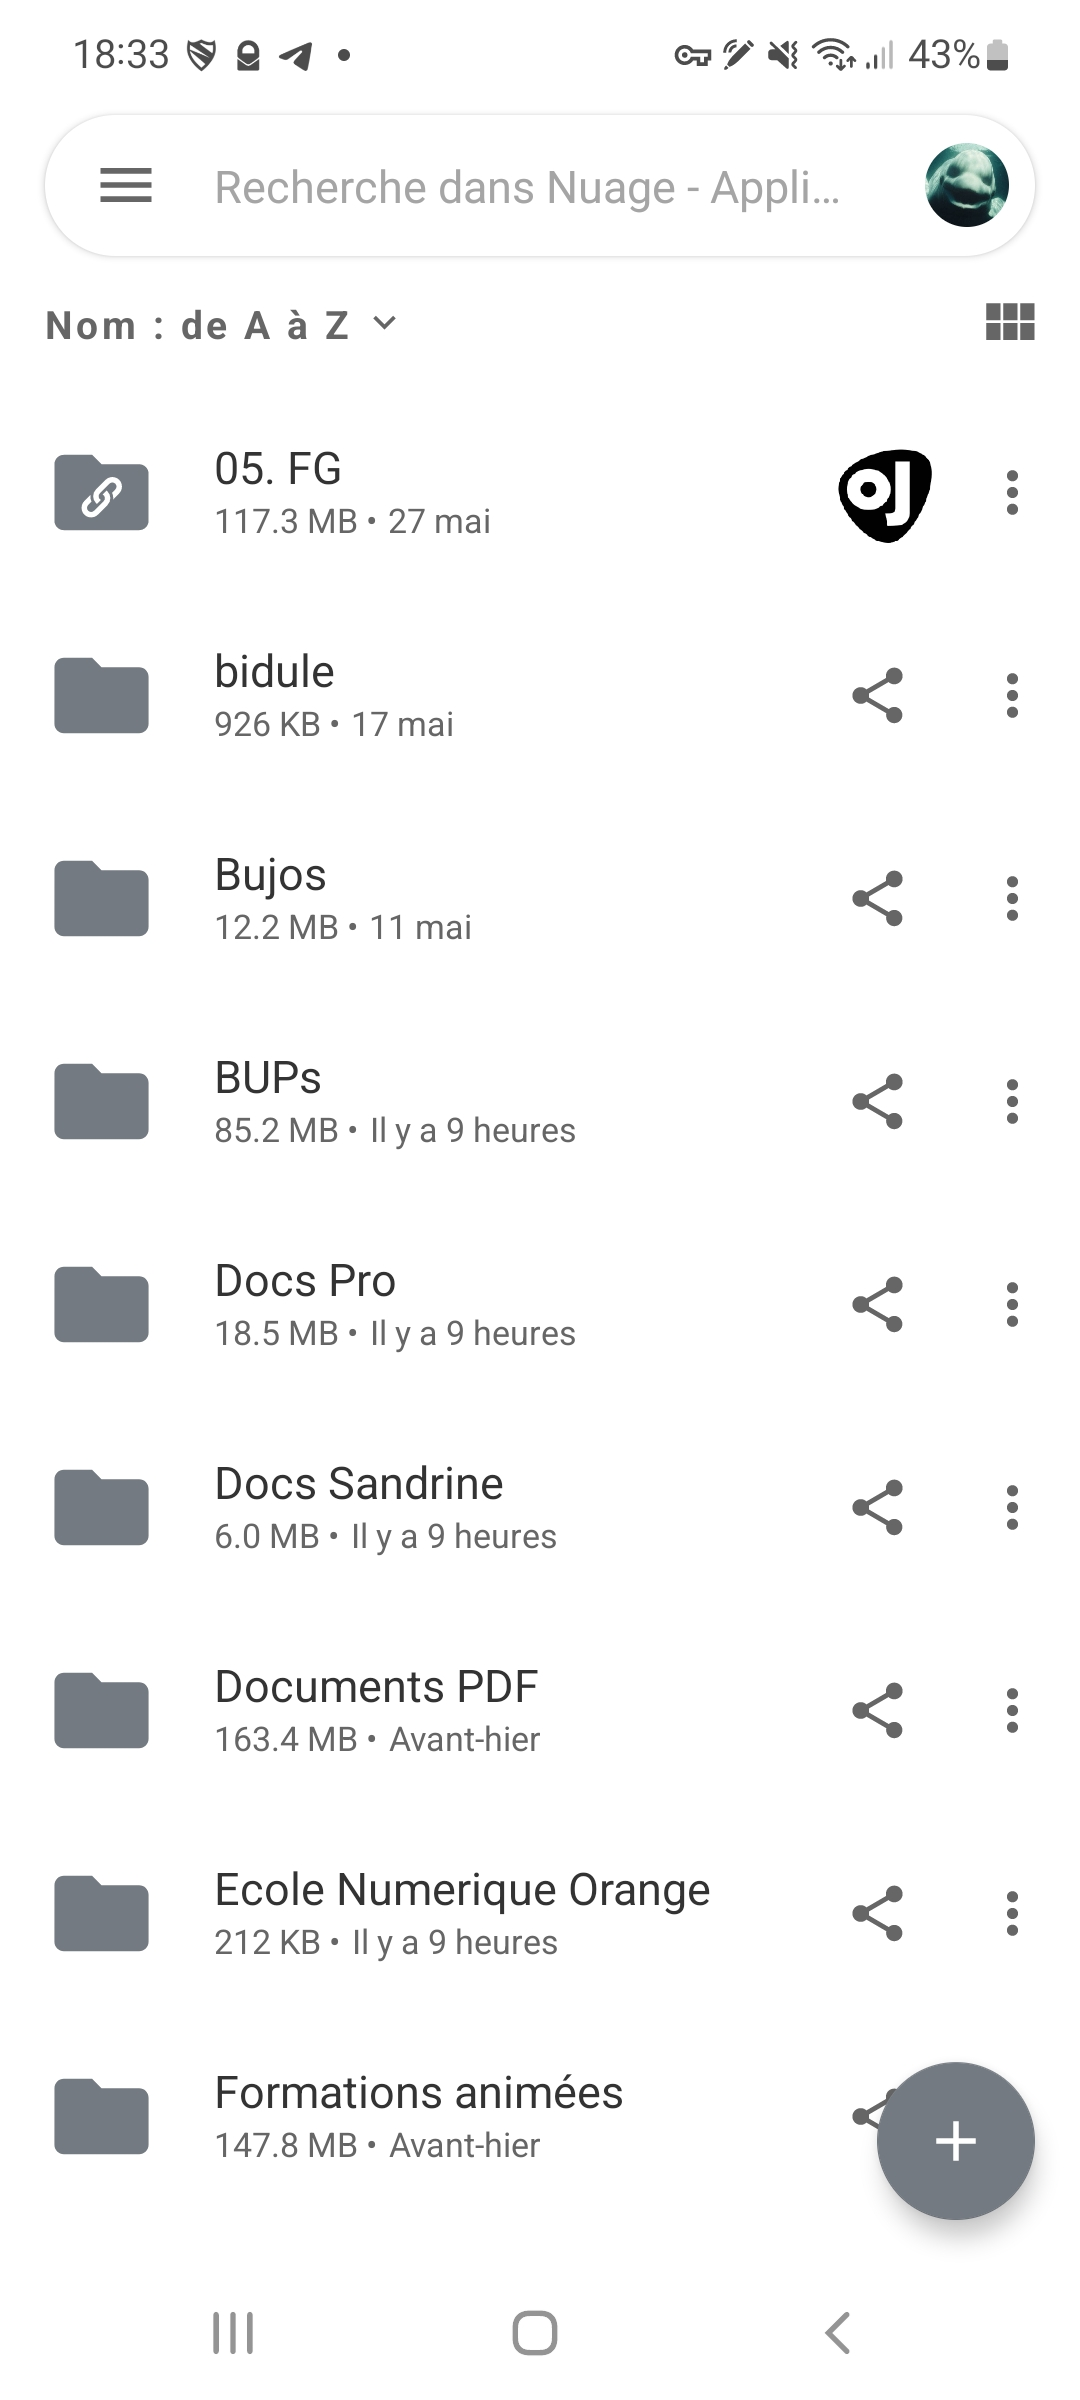
\includegraphics{./Captures/nextcloud-client.smartphone.jpg}
	\caption{Le client Nextcloud pour smartphone, version Android.}
\end{figure}
\end{multicols}
L'application est bien sûr disponible sur votre \emph{store\/}, quant au programme pour ordinateur il suffit d'aller sur le site \url{https://www.nextcloud.com} dans la section téléchargement.

Comment fonctionne le client Nextcloud pour PC~? 
C'est assez facile à comprendre. 
Lors de son installation, le client va demander un dossier, soit par défaut, soit en le spécifiant et en le créant, afin que tout fichier ou tout dossier qui y sera créé, supprimé, modifié, renommé, déplacé ou copié, sera synchronisé également sur le serveur automatiquement.
\begin{figure} \label{fig-dossier-synchro}
	\centering
	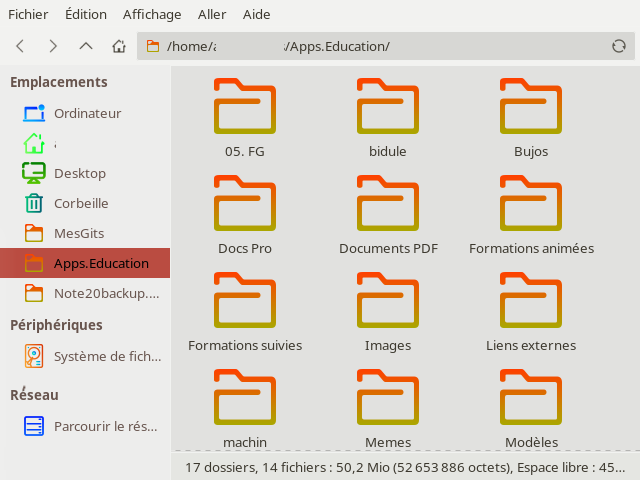
\includegraphics{./Captures/nextcloud-client.dossier.synchronise.png}
	\caption{Le dossier synchronisé sur mon P.C.}
\end{figure}

\paragraph{Notez.} 
Les prochaines sections et sous-sections traiteront de l'outil qui sera le plus souvent utilisé à savoir le transfert et la création d'objets par l'interface web, la gestion de tels échanges par le client nextcloud sera vu dans d'autres sections ultérieurement.

\section{Transfert de données}
%\addcontentsline{toc}{section}{Transfert de données}
Le transfert de fichiers et de dossiers entre périphériques est possible depuis plusieurs sources et selon plusieurs protocoles. 
L'image qui suit montre une synchronisation à double sens en utilisant le logiciel sur P.C. --~flèches en rose~--, ou bien via le navigateur --~flèches en bleu~-- ou encore via l'application d'un smartphone ou d'une tablette --~flèches en rouge.
\begin{figure}
	\centering
	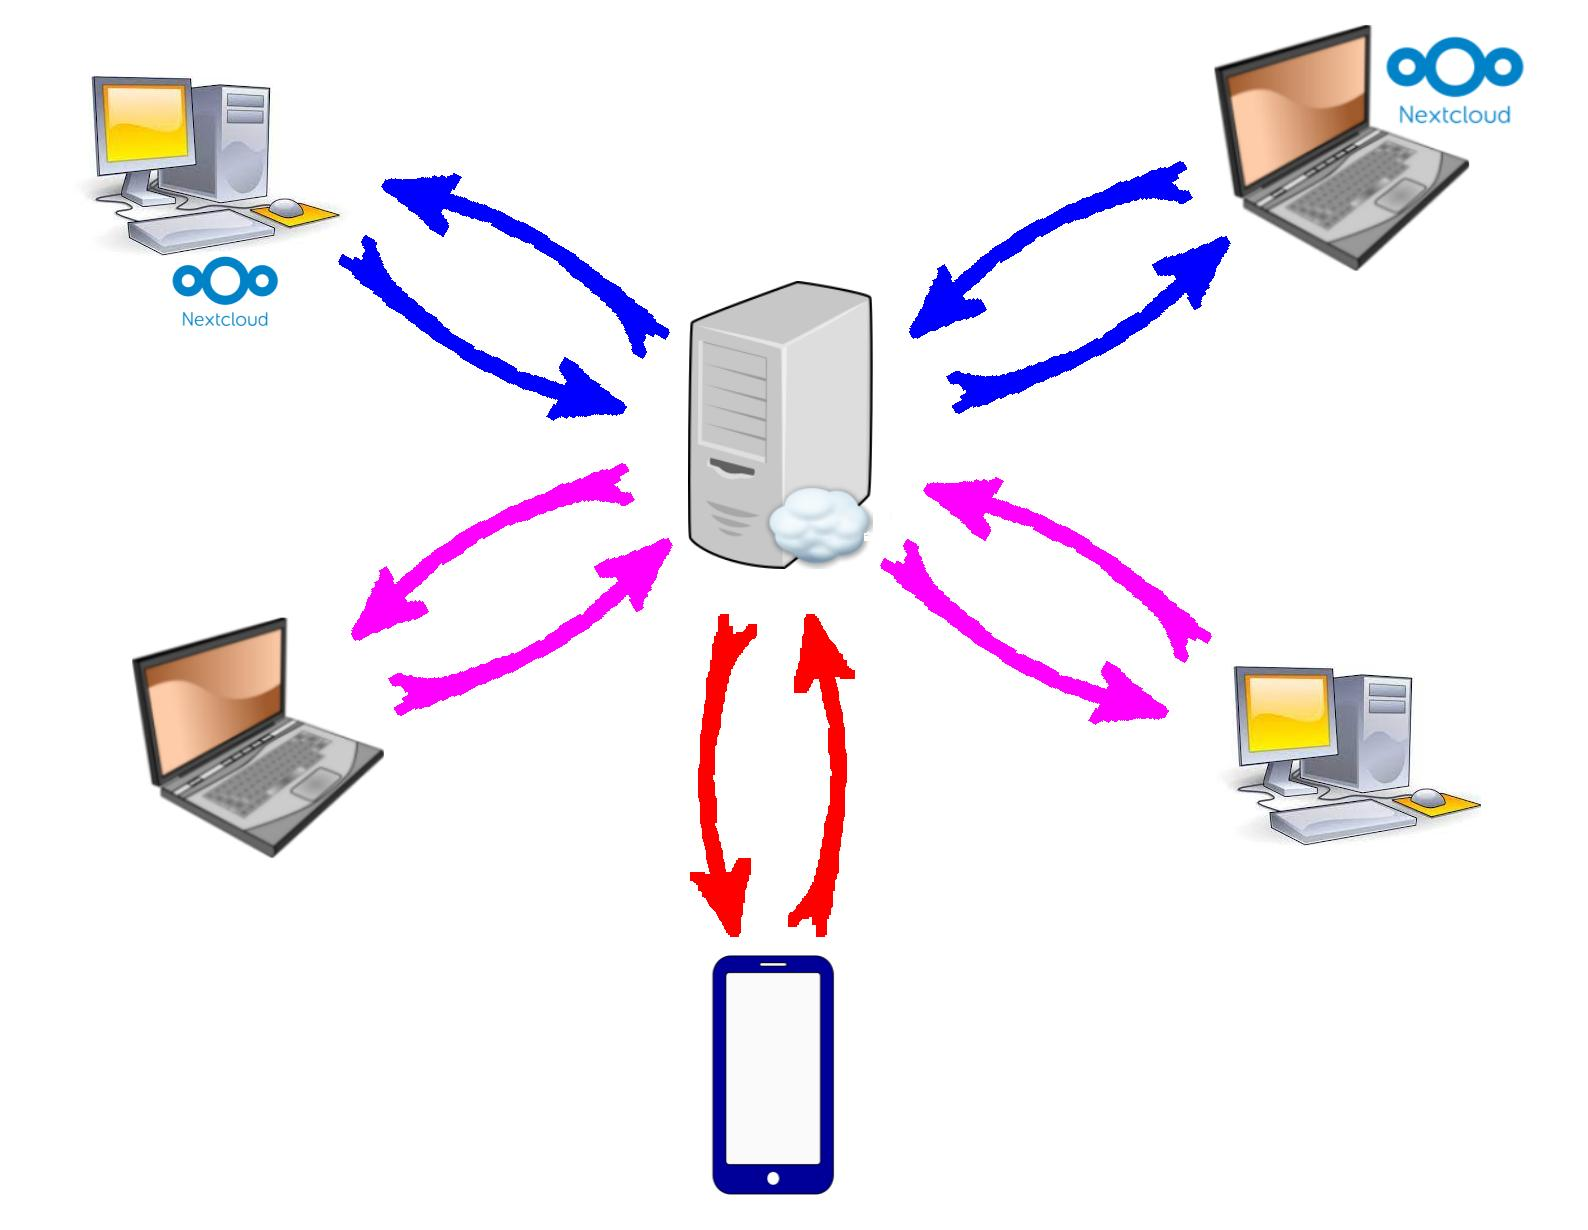
\includegraphics{./Captures/synchro.nextcloud.nuage.jpg}
	\caption{Le nuage est accessible par l'outil Nextcloud, par le navigateur, ou par le client smartphone pour transférer des données dans les deux sens.}
\end{figure}

\paragraph{La synchronisation via le client nextcloud pour ordinateur.} 
Comme le montre la capture d'écran du paragraphe \ref{fig-dossier-synchro}, transférer des fichiers entre l'ordinateur personnel et le nuage revient simplement à copier ou déplacer fichiers ou dossiers vers le dossier synchronisé, en soi on peut supposer que cette compétence est acquise par chaque lecteur.

Aussi dans les sous-sections suivantes ne seront abordés que le transfert de fichier par l'interface web.
De plus j'utiliserai le terme ``monter'' en lieu et place de l'anglicisme \emph{upload} et ``descendre'' parfois au lieu de télécharger.

\subsection{Monter un ou plusieurs fichiers}
%\addcontentsline{toc}{subsection}{Monter un ou plusieurs fichiers}
Tout se passe par l'icône en forme de rond avec une croix à l'intérieur, le {\Large $\oplus$} à gauche de la barre horizontale au dessus de l'espace réservé pour afficher les fichier. L'appui sur l'icône affiche le menu de la capture suivante~:
\begin{figure}
	\centering
	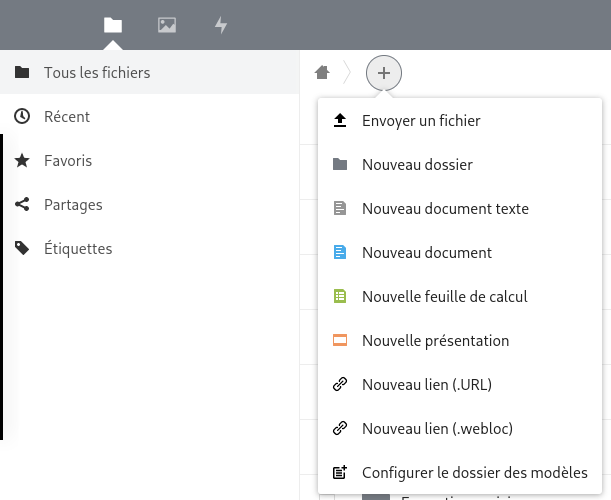
\includegraphics[width=0.5000\linewidth]{./Captures/nuage.menu.plus.png}
	\caption{Le menu ``plus''}
\end{figure}
En cliquant sur la ligne \og~Envoyer un fichier~\fg{} une fenêtre de l'explorateur local va s'ouvrir permettant de sélectionner un ou plusieurs fichiers qui seront envoyés dans le dossier affiché à l'écran.

\subsection{Créer un dossier}
%\addcontentsline{toc}{subsection}{Créer un dossier}
En cliquant sur la deuxième ligne du menu déroulant, c'est la création d'un dossier dans le dossier courant, attention il faut penser à clique sur la flèche au bout de la ligne pour valider le nom et créer le dossier.
\begin{figure}
	\centering
	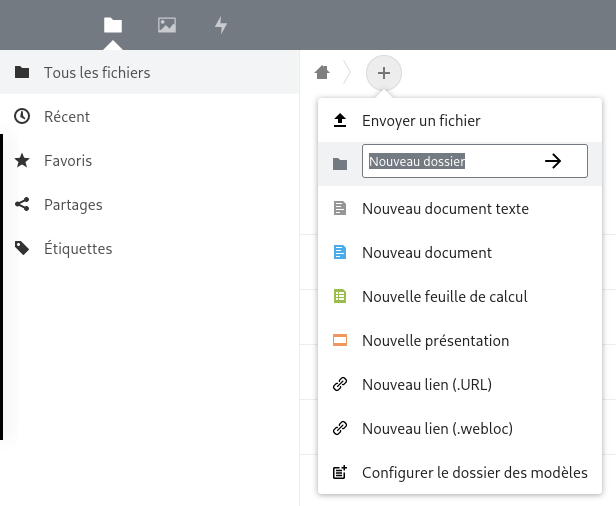
\includegraphics[width=0.5000\linewidth]{./Captures/nuage.menu.plus.creer.dossier.png}
	\caption{}
\end{figure}

Afin de valider la création d'un dossier, il suffit de saisir son nom et de valider par la touche entrée ou bien en cliquant sur la flèche en bout de ligne $\rightarrow$ et le dossier sera créé dans le dossier courant.

\subsection{Descendre un dossier ou plusieurs fichiers}
%\addcontentsline{toc}{subsection}{Descendre un dossier ou plusieurs fichiers}
L'un des avantages du nuage intégré à Apps.Education est la possibilité d'ouvrir, certes, mais aussi de télécharger ensuite un ou plusieurs fichiers, ou bien un ou plusieurs dossiers.

\begin{figure}
	\centering
	\includegraphics{./Captures/nuage.accueil.menu.contextuel.png}
	\caption{}
\end{figure}
Lorsqu'on appuie sur les \ldots un menu contextuel montre les différents choix proposés pour cet objet --~ici un fichier un texte balisé en langage \texttt{Markdown}. 

\subsection{Ce qui est spécifique au programme Nextcloud}
%\addcontentsline{toc}{subsection}{Ce qu'il n'est pas possible de faire} 
Par défaut, l'interface web du nuage ne permet pas d'envoyer directement un dossier, son contenu et toute la hiérarchie fille qui en découle, mais, cela reste possible par l'utilisation du client Nextcloud vu précédemment. 

Ouvrez deux fenêtres, l'une pointant le dossier synchronisé par le client Nextcloud, l'autre montrant la source des données à transférer, et, comme vous le feriez d'un dossier vers un dispositif externe, copiez ou déplacez les objets choisis (mélangeant tout ce que vous voulez de dossiers et de fichiers), quelques instants plus tard la synchronisation s'effectuera et créera dans le nuage les dossiers, les sous-dossiers et y placeront tous les fichiers quelque soit leur position dans l'arborescence.

Parmi les choix proposés, on peut renommer le fichier, le copier ou le déplacer --~c'est la même fenêtre mais pas le même bouton sur lequel cliquer~-- ou encore télécharger la ressource.

La règle est simple, si la ressource est un fichier simple, le fichier est téléchargé tel quel si par contre cela correspond à la sélection de plusieurs objets ou au moins d'un dossier, alors le nuage va compresser le tout dans une ressource unique, un fichier \emph{.zip} et c'est cet élément qui sera téléchargé.

\paragraph{Notez aussi.} 
On peut sélectionner un ou plusieurs objets en cliquant sur la case $\square$ en début de ligne, faisant apparaître en haut, à droite de \og~Nom~$\triangledown$~\fg{} comme le montre l'image qui suit.
\begin{figure}
	\centering
	\includegraphics{./Captures/nuage.selection.plusieurs.objets.png}
	\caption{Sélection de plusieurs objets}
\end{figure}
on peut aussi sélection tous les objets du répertoire en cliquant sur le $\square$ tout en haut.
\begin{figure}
	\centering
	\includegraphics{./Captures/nuage.selection.tous.objets.png}
	\caption{Sélection complète}
\end{figure}

\section{Partager une ressource}
%\addcontentsline{toc}{section}{Partager une ressource} 
Tout document posé dans le nuage, que ce soit un simple fichier ou bien un dossier à un ou plusieurs sous-niveaux est une ressource pouvant être partagée. 
Les limitations imposées par les choix collaboratifs font que pour l'heure il est impossible de partager une ressource vers un groupe d'utilisateurs directement, il faut partager utilisateur après utilisateur. 
Malgré cela, le partage reste une fonctionnalité fort utile.

\subsection{Partage simple}
%\addcontentsline{toc}{subsection}{Partage simple}
Il est possible
\begin{itemize}
    \item Vers un utilisateur,
    \item Vers plusieurs utilisateurs, en partageant la même ressource utilisateur après utilisateur,
    \item Vers le public.
\end{itemize}

\paragraph{Comment apparaissent les ressources partagées ?}
Dans l'espace m'étant alloué plusieurs ressources sont déjà partagées, provenant d'autres utilisateurs ou bien étant partagées par moi vers d'autres.
\begin{figure}
	\centering
	\includegraphics{./Captures/nuage.partager.icones.png}
	\caption{Deux exemples de ressources partagées et deux autres non partagées.}
\end{figure}
Ainsi, le dossier \og~O5 FG~\fg{} a été utilisé par un autre utilisateur dont les initiales sont OJ (puisqu'aucun avatar ne semble avoir été défini par l'utilisateur). 
Le dossier \og~BUPs~\fg{} par contre fait l'objet d'un partage de ma part. 
Il est intéressant de noter que les icônes représentant ces deux ressources et les deux autres (Bidule et Bujos) diffèrent et que suivant le sens du partage le motif superposé à l'icône n'est pas le même. 

\subsection{Les options de partage avancées}
%\addcontentsline{toc}{subsection}{Les options du partage}
Pour avoir  plus de détails il suffit soit de cliquer sur l'icône \ldots soit sur l'icône de partage et alors le volet latéral des propriétés de partage apparaîtra.
\begin{figure}
	\centering
	\includegraphics{./Captures/nuage.partager.menu.contextuel.png}
	\caption{Les différentes possibilités de partage offertes.}
\end{figure}

On voit par la dernière capture qu'il est possible de gérer les droits de modification, de création ou de suppression sur la ressource, mais aussi d'autoriser le repartage et, plus intéressant encore, de définir un mot de passe d'accès et une date d'expiration du partage.

\section{Créer un lien vers une ressource extérieure.}
Il peut être pratique de conserver sous forme de fichier un lien vers une ressource internet. 
Dans mon établissement ce type de fichier m'est très pratique pour déployer sur tous les postes accueillant les évaluations des élèves de 6\ieme{} en utilisant un fichier sur un espace de stockage partagé en interne dans l'établissement et en le copiant de poste en poste --nous n'avons pas de domaine, ni de politique de déploiement par GPO-- du coup le fichier \texttt{.url} contient le lien qui sera ouvert par le navigateur par défaut de la machine vers le site web de passation des épreuves. 

%\newpage % force le passage sur une nouvelle page pour que les colonnes restent bien comme il faut, au besoin
\begin{multicols}{2}
Tout commence par le menu $\oplus$ \ldots
\begin{figure}
	\centering
	\includegraphics{./Captures/nuage.menu.plus.zoom.png}
	\caption{Le menu $\oplus$.}
\end{figure}
\columnbreak

Je sélection la ligne pour les URL.
\begin{figure}
	\centering
	\includegraphics{./Captures/nuage.menu.plus.creer.url.png}
	\caption{Nommage du raccourcis}
\end{figure}
\end{multicols}

Je choisis de nommer par \texttt{nom-du-fichier} le fichier \texttt{.URL} qui sera généré, il contiendra un lien vers le site \url{https://ctan.org}~:
\begin{figure}
	\centering
	\includegraphics[width=0.333\linewidth]{./Captures/nuage.url.proprietes.png}
	\caption{Les propriétés du lien.}
\end{figure}

et je règle les options relatives à son ouverture (même fenêtre, fenêtre de confirmation, \ldots), ce qui fait qu'en cliquant sur le lien, la mini fenêtre suivante va s'afficher :
\begin{figure}
	\centering
	\includegraphics[width=0.333\linewidth]{./Captures/nuage.url.fenetre.confirmation.png}
	\caption{Confirmation de l'ouverture du lien.}
\end{figure}

Le site s'ouvre alors dans un nouvel onglet conformément aux propriétés réglées antérieurement.
\begin{figure}
	\centering
	\includegraphics{./Captures/nuage.url.ouverture.nouvel.onglet.png}
	\caption{Le site CTAN.org est désormais ouvert dans un nouvel onglet.}
\end{figure}

\section{Libreoffice \emph{online}}

Au sein du nuage, \emph{LibreOffice OnLine\/} ou encore LOOL a été intégrée, toujours dans le menu $\oplus$ et offre le traitement de textes \emph{writer\/}, le tableur \emph{calc\/} et le logiciel de présentation \emph{impress\/}, permettant d'ouvrir les document montés sur le nuage mais aussi d'éditer ceux déjà présents.

Ainsi vous accéderez aux trois outils de la suite bureautique libreoffice online les plus utilisés, le traitement de textes \emph{writer\/}, le tableur \emph{calc\/} et le logiciel de présentations \emph{impress\/} comme le montrent les captures suivantes.

\begin{figure}
    \centering
    \includegraphics[]{Captures/nuage.lool.writer.png}
    \caption{Exemple de fichier de traitement de textes composé dans Libreoffice \emph{writer\/} au sein du nuage.}
\end{figure}

La capture d'écran ci-avant montre un document rédigé entièrement en ligne, inclusion d'image comprise, avec le volet latéral de Libreoffice actif.

Il faut prendre en compte quelques points néanmoins, l'un d'entre eux est qu'à l'instar de la suite \emph{Office\/} de Microsoft\textregistered{} la version en ligne n'est pas complète mais une version allégée. 
Les utilisateurs avancés de Libreoffice se verront amputés de quelques fonctionnalités, par exemple en ce qui me concerne, l'éditeur d'équations.
Notez cependant qu'un fichier édité en local, \emph{i.e.\/} sur un ordinateur directement par la version complète de Libreoffice sera conservé lors du transfert, et, s'il y a ouverture, sera considéré comme un objet inséré dans le document malgré l'impossibilité d'éditer directement son contenu.

\begin{figure}
    \centering
    \includegraphics[]{Captures/nuage.lool.tableur.png}
    \caption{Un exemple de tableur/grapheur sous Libreoffice \emph{Calc\/} et un graphique inséré, le tout directement en ligne.}
\end{figure}

Le tableur permet l'édition de formules et l'insertion de graphiques, comme on pouvait l'espérer.

\begin{figure}
    \centering
    \includegraphics[]{Captures/nuage.lool.presentation.png}
    \caption{Une ébauche de présentation de Libreoffice \emph{Impress\/} en plein développement.}
\end{figure}

Et évidemment il est possible de créer des présentations simples voire complexes le tout en ligne, ou de les modifier.

La suite bureautique Libreoffice Online permet aussi d'exporter, et \emph{de facto} de télécharger les documents produits dans divers formats, l'exemple suivant montre les exportations associées à \emph{Writer\/}.

\begin{figure}
    \centering
    \includegraphics[]{Captures/nuage.lool.writer.exportations.png}
    \caption{Les exportations proposées dans Libreoffice \emph{writer\/}.}
\end{figure}

Cette fois-ci vous aurez noté que le volet latéral est occulté.

% Chapitre sur l'agenda
\chapter{L'agenda.}
%\addcontentsline{toc}{chapter}{L'agenda}

\begin{figure}
    \centering
    \includegraphics{Captures/agenda.jour.png}
\end{figure}

\begin{figure}
    \centering
    \includegraphics{Captures/agenda.semaine.png}
\end{figure}

\begin{figure}
    \centering
    \includegraphics{Captures/agenda.semaine.we.png}
\end{figure}



% Chapitre remerciements-notices-legales
\chapter*{Remerciements et informations légales}
%\addcontentsline{toc}{chapter}{Remerciements et informations légales}

Ce document a été entièrement réalisé avec les langages de balisage \texttt{Markdown} et \LaTeX{}. 
Il a été rédigé avec un bloc-notes (\texttt{mousepad}) et un éditeur \LaTeX{} (\texttt{\TeX{}maker}), tous deux logiciels libres de droits.
Les captures d'écran ont été réalisées avec le logiciel \texttt{xfce4-screenshooter} et modifiées par un éditeur basique tel que \texttt{Kolourpaint}

\newpage
\renewcommand{\baselinestretch}{1}
\setlength{\parskip}{0em}
\tableofcontents

\end{document}